% *********************************************************
% Check "thesis-style.sty" to customise language and others
% *********************************************************

\documentclass[a4paper,12pt,twoside]{ThesisStyle}
\usepackage{thesis-style}
\usepackage[utf8]{inputenc}
\usepackage{enumitem}

\newcommand{\titlemark}{Desenvolupament d’una aplicació òbil de codi obert per a fer pagaments entre usuaris mitjaçant codis QR} % Project title for custom header
\newcommand{\documentmark}{Memòria} % Document type for custom header
\newcommand{\appendixmark}{Annex} % Appendix mark for custom header

% \cftsetindents{section}{1em}{3em}
% \setlength\cftsectionnumwidth{4em} % uncomment to see difference

\begin{document}

\frontmatter

\pagenumbering{gobble}

\thispagestyle{empty}
\begin{table}[htb]
\centering
\begin{Large}
\resizebox{\textwidth}{!}{\begin{tabular}{ | l |}
 \hline
 \\

\includegraphics[scale=0.9]{imatges/logo_eps.png} \\[0.7cm]
\centerline{Projecte fi de grau}\\[1cm]
\hline
\\
Estudi: Grau en Enginyeria Informàtica\\[0.7cm]
\hline
\\
Títol: Desenvolupament d'una aplicació mòbil de codi obert per a fer pagaments\\
entre usuaris mitjaçant codis QR\\[0.7cm]
\hline
\\
Document: Memòria\\[0.7cm]
\hline
\\
Alumne: Sudan Wu\\[0.7cm]
\hline
\\
Tutor: Pau Xiberta i Armengol\\
Departament: INFORMÀTICA, MATEMÀTICA APLICADA I ESTADÍSTICA\\
Àrea: LLENGUATGES I SISTEMES INFORMÀTICS\\[0.7cm]
\hline
\\
Convocatòria (Setembre/2024): XXX\\[0.7cm]
\hline

\end{tabular}}
\end{Large}
\end{table}

\newpage

\begin{titlepage}

% Upper part of the page

\includegraphics[scale=0.9]{imatges/logo_eps.png} \\[1cm]
\begin{center}
\textsc{\Large Projecte Fi de Grau} \\[1cm]

% Title
\begin{spacing}{2}
\HRule \\
\textbf{\Huge Títol del projecte} \\
\HRule \\[0.5cm]
\end{spacing}

% Author and supervisor and other data
{
\large
\emph{Autor:} \\
Nom \textsc{Sudan Wu} \\[1cm]
Setembre 2024 \\[1cm]
Grau en Enginyeria Informàtica \\[1cm]
\emph{Tutor:} \\
Nom \textsc{Pau Xiberta i Armengol} \\
}

\end{center}
\end{titlepage}

\titlepage

\dominitoc

\pagenumbering{roman}

\chapter*{Resum}
\label{chp:resum}


Aquest projecte té com a objectiu desenvolupar una aplicació innovadora que permeti realitzar transaccions bancàries de manera ràpida, segura i flexible mitjançant codis QR. Inspirat en la meva experiència a la Xina, on les aplicacions de pagament integrades en plataformes com WeChat són omnipresents, aquest sistema pretén simplificar les operacions bancàries substituint les màquines TPV tradicionals. D'aquesta manera, s'elimina la necessitat d'invertir en hardware addicional i es redueixen els costos associats amb la infraestructura de pagament. Aquesta solució no només simplifica el procés de pagament, sinó que també ofereix una alternativa moderna i tecnològicament avançada a les màquines TPV (Terminal Punt de Venda) tradicionals, contribuint així a una experiència de pagament més fluida i sense interrupcions.\\

A llarg termini, el sistema té el potencial d'evolucionar, ja sigui com a funcionalitat incorporada a les aplicacions bancàries existents o com a plataforma de pagament independent similar a PayPal. Les funcionalitats futures podrien incloure un sistema d'anàlisi de transaccions, pagaments recurrents, millores visuals, notificacions per veu... El projecte posa un èmfasi especial en la seguretat, amb l'objectiu de millorar la protecció de les dades utilitzant tecnologies d'encriptació avançades.\\

Aquest sistema està dissenyat per ser escalable, adaptable tant a petits comerços com a grans empreses, i preparat per a un futur on els pagaments digitals continuïn creixent en importància.





\chapter*{Agraïments}
\label{chp:agraiments}

Per començar vull agrair molt especialment a al meu tutor Pau Xiberta i Armengol, per la seva guia, paciència i saviesa durant tot el procés. Les seves orientacions han estat fonamentals per a la consecució d’aquest treball, i la seva dedicació ha estat una font constant de motivació.\\

També voldria agrair als meus companys i amics per estar sempre al meu costat, oferint suport emocional i consells valuosos en moments de dubte i incertesa. La vostra companyia ha fet aquest viatge molt més suportable i enriquidor.\\

No puc oblidar la meva família, que ha estat el meu pilar més ferm al llarg de tota aquesta etapa acadèmica. Gràcies per creure en mi, per la vostra paciència infinita i per animar-me a seguir endavant, fins i tot en els moments més difícils.\\

Finalment, vull reconèixer l’esforç i dedicació de tots els professors que m’han format durant aquests anys. Les vostres ensenyances han estat fonamentals per arribar fins aquí, i cada una de les vostres lliçons ha deixat una petjada en aquest treball.\\

A tots, gràcies de tot cor per fer possible aquest assoliment.


\tableofcontents

\listoffigures

\listoftables

\mainmatter



\chapter{Introducció, motivació, finalitat i objectius del projecte}
\label{chp:intro}

\section{Introducció}
\label{sec:Introduccio}

A l'hora de processar un pagament, la majoria de botigues utilitzen un Terminal Punt de Venda (TPV) físic, i els clients fan servir una targeta bancària o una cartera digital que incorpora aquesta targeta. El TPV actua com a intermediari en l'operació, introduint un procés addicional que pot augmentar tant els costos com el risc d'errors. Tot i que existeixen plataformes de pagament en línia, aquestes no estan dissenyades per substituir completament el TPV físic, i sovint no són de codi obert ni ofereixen l'opció de realitzar transaccions mitjançant codis QR.

\section{Motivació}
\label{sec:Motivacio}

L’evolució tecnològica i la digitalització han transformat profundament la manera com les empreses gestionen els seus processos de pagament. Tot i els avenços, el sistema tradicional basat en terminals físics de punt de venda (TPV) encara predomina, arrossegant amb si costos operatius elevats i riscos associats a errors humans i fraus. Aquesta situació, sumada a la creixent adopció de tecnologies de pagament mòbil i l’ús de codis QR en diverses parts del món, posa de manifest la necessitat d’explorar alternatives més eficients, segures i accessibles.\\

Aquest projecte neix de la voluntat d’abordar aquestes limitacions, oferint una solució que pugui substituir o complementar els TPV físics amb una plataforma de pagament en línia de codi obert. Una solució que permeti als comerciants processar transaccions mitjançant codis QR, oferint així una experiència de pagament més ràpida, senzilla i segura tant per a les botigues com per als clients.\\

La motivació principal d’aquest projecte és reduir els costos operatius i minimitzar els riscos associats als sistemes de pagament tradicionals, alhora que es promou la inclusió tecnològica a través d’una eina de codi obert, accessible per a qualsevol empresa o desenvolupador que desitgi implementar-la. Creiem que, mitjançant aquesta iniciativa, podem contribuir a la transformació digital del comerç, afavorint la seva competitivitat i adaptabilitat en un mercat cada cop més globalitzat i dinàmic.

\section{Finalitat i objectius del projecte}
\label{sec:Finalitat i objectius del projecte}

L'objectiu d'aquest treball de final de grau és desenvolupar una aplicació full stack que inclogui totes les funcions necessàries per gestionar pagaments mitjançant codis QR. Aquest desenvolupament inclourà:

\begin{itemize}
  \item El disseny i la implementació de la base de dades per emmagatzemar la informació de les transaccions i els usuaris.
  \item El desenvolupament d'una API que permeti interactuar de manera eficient amb la base de dades, facilitant la creació, gestió i consulta de pagaments.
  \item La creació d'una interfície d'usuari senzilla i intuïtiva, que permeti als usuaris generar i escanejar codis QR per realitzar transaccions.
  \item El desenvolupament de les aplicacions frontals basades en aplicacions que permetin als usuaris accedir al sistema, generar codis QR i realitzar els pagaments de manera segura i ràpida.
\end{itemize}

L'aplicació permetrà als clients generar codis QR tant per realitzar pagaments com per rebre cobraments, que podran ser escanejats amb qualsevol dispositiu que tingui càmera per completar la transacció.


\chapter{Viabilitats}
\label{chp:viabilitats}

\section{Introducció}
\label{subsec: Introducció}

L'estudi de la viabilitat del projecte es tindrà en compte des de la tècnica
recursos, cost econòmic del projecte i viabilitat del mercat.\\

En conjunt demostra que el projecte és viable i té un alt potencial de creixement en l'entorn actual, oferint una solució innovadora i segura per als pagaments mòbils a través de codis QR.

\section{Viabilitat tècnica}
\label{subsec:Viabilitat tècnica}

L’aplicació utilitzarà Node.js i Apollo Server per a la gestió del servidor, mentre que Flutter s’emprarà per al desenvolupament de la interfície d’usuari. A més, es farà servir una base de dades en MongoDB Cloud per emmagatzemar les transaccions i la informació dels usuaris. Aquestes tecnologies són àmpliament utilitzades i compten amb un ampli suport per part de la comunitat de desenvolupadors.

\section{Viabilitat econòmica}
\label{subsec:Viabilitat económica}

Els costos principals del projecte inclouen el desenvolupament de l'aplicació, que es realitzarà internament, i els costos d'allotjament en el núvol, que seran proporcionats per serveis com AWS amb un pressupost de X euros mensuals.\\

\begin{figure}[h!] % La posició de la figura pot ser ajustada amb 'h!', 't', 'b', etc.
    \centering
    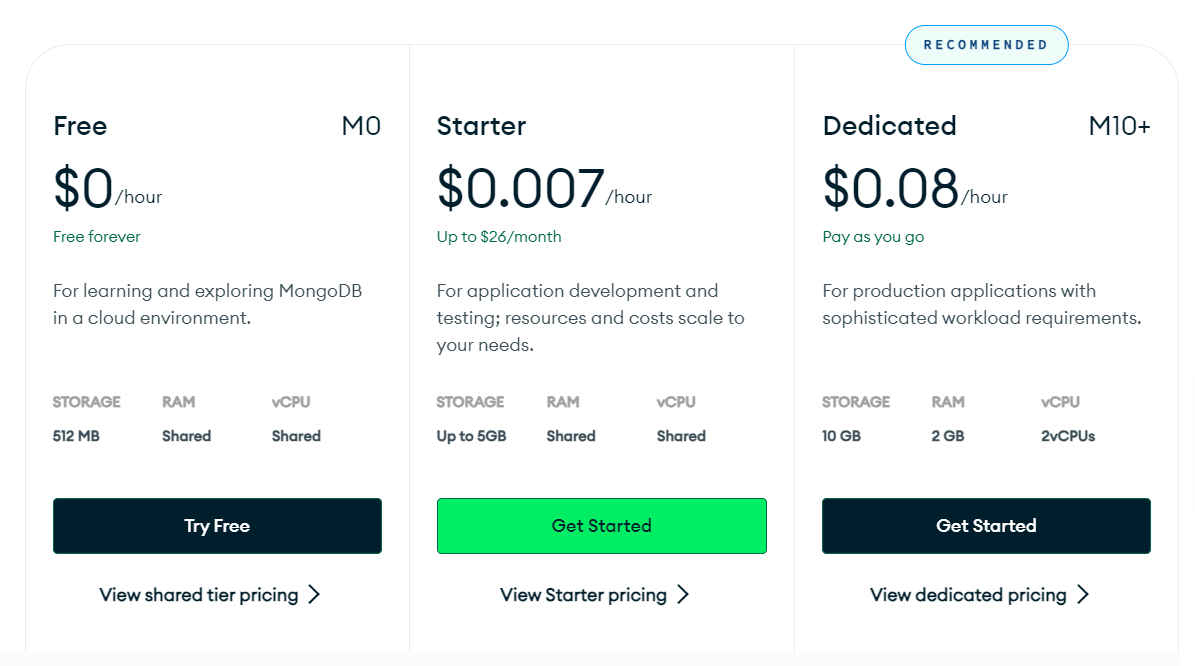
\includegraphics[width=0.8\textwidth]{imatges/mongodb.png} % Ajusta el nom i el camí del fitxer d'imatge
    \caption{El preu del servei MongoDB Atlas} % Títol de la imatge
    \label{fig:El preu del servei MongoDB Atlas} % Etiqueta per referenciar la imatge
  \end{figure}

El sistema de pagament mitjançant codis QR ofereix una solució econòmica en comparació amb els terminals de TPV tradicionals, amb una possible font d'ingressos a través de comissions per transacció i opcions de subscripció per serveis addicionals.



\section{Viabilitat de mercat}
\label{subsec:Viabilitat de mercat}

Amb l'augment de l'ús de pagaments mòbils i la necessitat de solucions de pagament contactless, hi ha una demanda creixent per a sistemes de pagament basats en codis QR. Aquesta tendència proporciona una oportunitat significativa per a la nostra aplicació.\\

Encara que hi ha altres solucions de pagament basades en codis QR, el nostre sistema es diferencia per la seva integració fàcil amb altres plataformes i la seva estructura de codi obert, que permet personalització i adaptació a les necessitats específiques dels usuaris.

\begin{figure}[h!] % La posició de la figura pot ser ajustada amb 'h!', 't', 'b', etc.
    \centering
    
\includegraphics[width=0.3\textwidth]{imatges/paypal.png} % Ajusta el nom i el camí del fitxer d'imatge
    \caption{Un codi QR de Paypal} % Títol de la imatge
    \label{fig:Un codi QR de Paypal} % Etiqueta per referenciar la imatge
  \end{figure}



\chapter{Metodologia}
\label{chp:metodologia}


\section{Introducció}
\label{subsec: Introducció}

La metodologia utilitzada en aquest projecte és àgil Scrum, tot i que es tractava d'un projecte individual. 

\section{Scrum}
\label{subsec: Scrum}

Scrum és un marc de treball per a la gestió de projectes, conegut per la seva flexibilitat i per permetre gestionar projectes complexos a través de cicles iteratius de treball anomenats sprints. Encara que tradicionalment Scrum està dissenyat per a equips, es van adaptar els seus principis per optimitzar la gestió del temps i els recursos durant el desenvolupament del projecte.\\

\begin{figure}[h!] % La posició de la figura pot ser ajustada amb 'h!', 't', 'b', etc.
  \centering
  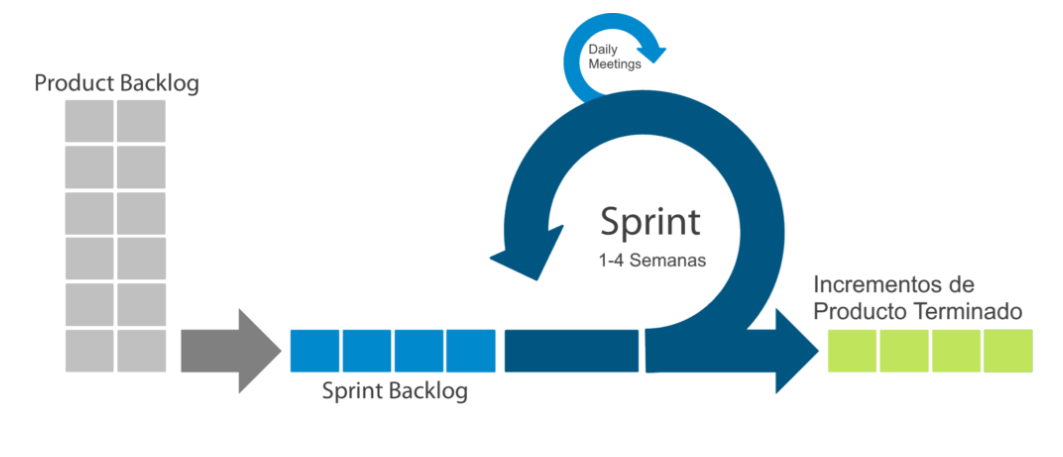
\includegraphics[width=0.8\textwidth]{imatges/scrum.png} % Ajusta el nom i el camí del fitxer d'imatge
  \caption{Sistema de treball Scrum} % Títol de la imatge
  \label{fig:Sistema de treball Scrum} % Etiqueta per referenciar la imatge
\end{figure}

L'elecció de Scrum es va basar en la necessitat de mantenir una alta capacitat de resposta davant els canvis en els requisits i per estructurar el procés de desenvolupament en fases manejables. Scrum va permetre dividir el projecte en sprints, cosa que va facilitar la planificació i el seguiment del progrés, assegurant-se que cada fase del projecte es completava abans de passar a la següent.\\

Per a la planificació del projecte, es defineixen sprints de dues setmanes, cadascun amb objectius específics que cal complir abans d’iniciar el següent sprint. Al principi de cada sprint, s’elabora un pla detallat de les tasques a realitzar, prioritzant les més crítiques i assegurant que estan alineades amb els objectius generals del projecte.\\

Es crea i es gestiona un product backlog que llista totes les funcionalitats a desenvolupar. Aquest backlog es prioritza d’acord amb la seva importància i la complexitat de la implementació. Cada sprint es planifica tenint en compte aquesta llista, garantint que es treballa sempre en les tasques més rellevants per al progrés del projecte.\\

L'ús de Scrum, adaptat a un entorn individual, va ser fonamental per a la gestió eficient del temps i la consecució dels objectius del projecte. Va permetre que el desenvolupament es realitzés de manera ordenada i progressiva, proporcionant la flexibilitat necessària per fer ajustos sobre la marxa. Aquesta metodologia va resultar especialment útil per mantenir el ritme de treball i assegurar que cada fase del projecte es completés amb èxit abans de passar a la següent.



\chapter{Planificació}
\label{chp:planificació}

\section{Introducció}
\label{sec:Introducció}

El següent pla de planificació ofereix una visió clara del procés de desenvolupament del projecte, destacant les etapes clau, el temps assignat i els resultats esperats, així com l'aplicació de la metodologia Scrum per gestionar el projecte de manera àgil.



\section{Desenvolupament}

El procés de creació i construcció del producte de programari inclou les següents tasques:

\begin{enumerate}
  \item \textbf{Anàlisi de Requisits}:
  \begin{itemize}
      \item Revisar els requisits del projecte.
      \item Establir especificacions detallades per al desenvolupament.
  \end{itemize}

  \item \textbf{Disseny}:
  \begin{itemize}
      \item Crear l'arquitectura del sistema.
      \item Dissenyar les interfícies d'usuari i les interaccions.
      \item Definir les estructures de dades i les lògiques d'operació.
  \end{itemize}

  \item \textbf{Codificació}:
  \begin{itemize}
      \item Escriure el codi font segons les especificacions.
      \item Implementar les funcionalitats del sistema.
      \item Desenvolupar codi de backend amb Apollo-server i frontend amb Flutter
  \end{itemize}

  \item \textbf{Proves}:
  \begin{itemize}
      \item Crear i executar proves per verificar la funcionalitat de cada component.
      \item Corregir errors detectats durant les proves.
  \end{itemize}

  \item \textbf{Revisió de Codi}:
  \begin{itemize}
      \item Realitzar revisions de codi per assegurar la qualitat i el compliment dels estàndards.
  \end{itemize}

  \item \textbf{Documentació}:
  \begin{itemize}
      \item Elaborar memòria sobre l’arquitectura, el disseny i el codi.
  \end{itemize}

  \item \textbf{Manteniment i Actualitzacions}
    \begin{itemize}
        \item Realitzar manteniment regular del sistema per assegurar la seva funcionalitat.
        \item Implementar actualitzacions i millores basades en feedback i nous requisits.
    \end{itemize}


\end{enumerate}


\subsection{Calendari previst}
\label{subsec: Calendari previst}

\begin{table}[h!]
\centering
\begin{tabular}{|c|c|c|c|c|}
\hline
\textbf{Núm.} & \textbf{Fase} & \textbf{Data d'Inici} & \textbf{Data de Finalització} & \textbf{Resultats}\\
\hline
1 & Anàlisi de Requisits & 01/04/2024 & 07/04/2024 & ok \\
2 & Disseny & 08/04/2024 & 21/04/2024 & ok\\
3 & Codificació & 22/04/2024 & 30/06/2024 & ok\\
5 & Proves & 01/07/2024 & 15/07/2024 & ok\\
6 & Revisió de Codi & 16/07/2024 & 31/07/2024 & ok\\
7 & Documentació & 01/08/2024 & 31/08/2024 & ok\\
8 & Manteniment i Actualitzacions & 01/09/2024 & Continu & ok\\
\hline
\end{tabular}
\caption{Calendari del projecte}
\label{tab:calendari}
\end{table}



\chapter{Marc de treball i conceptes previ}
\label{chp:marcdetreball}


\section{Introducció}
\label{subsec:Introducció}

En aquest capítol es tractaran els coneixements necessaris per desenvolupar correctament una aplicació bancària que utilitza codi QR per realitzar operacions. En resum, és important entendre com funciona el codi QR, especialment en relació amb com emmagatzemar el contingut. A més, cal disposar de coneixements sobre arquitectura i desenvolupament de programari per aportar valor a l'aplicació.

\subsection{Propòsit}
\label{subsec: Propòsit}

L'objectiu de l'aplicació és proporcionar una plataforma senzilla, escalable i potent per gestionar els pagaments i cobraments mitjançant codis QR. Tant els clients com els comerciants tindran accés a funcionalitats i permisos dins de l'aplicació, permetent-los configurar els seus sistemes de pagament o cobrament, establir opcions disponibles, ajustar els límits de transacció i altres configuracions relacionades. A més de facilitar les compres, l'aplicació permetrà als usuaris realitzar transferències entre amics i familiars, oferint així una solució versàtil per a diverses necessitats financeres quotidianes.\\

Per tant, en una sola aplicació, els usuaris podran controlar totes les transaccions que es realitzin, alhora que tindran la capacitat d'aplicar canvis i modificacions segons les seves necessitats i preferències.\\


A continuació, es presenta una llista amb les parts fonamentals que defineixen el funcionament de l'aplicació:

\begin{itemize}
    \item App: L'aplicació es pot concebre com una entitat bancària en si mateixa, on els seus usuaris actuen com a clients que poden tant rebre com enviar pagaments. 
    \item Usuari - Client: L'usuari client és la persona que utilitza l'aplicació per realitzar pagaments o cobraments.
    \item Usuari - Administrador: L'usuari administrador és qui gestiona l'aplicació, configurant els sistemes de pagament i supervisant les transaccions, comptes i també els usuaris.
    \item Codi QR: El codi QR és un element clau de l'aplicació, utilitzat per comunicar informació entre clients.

\end{itemize}



\subsection{Codi QR}
\label{subsec: Codi QR}

Els codis QR (Quick Response) van ser desenvolupats al Japó a mitjans dels anys 90, és un tipus de codi de barres bidimensional que pot emmagatzemar una gran quantitat d'informació en un espai reduït. Aquest codi es pot escanejar fàcilment amb la càmera d'un telèfon mòbil o amb dispositius específics, permetent accedir a la informació que conté de manera ràpida i senzilla.\\

La imatge següent mostra un codi QR. Es pot escanejar amb la càmera del mòbil i conté text emmagatzemat en el seu interior. El codi QR té tres quadrats grans en les cantonades, que ajuden a posicionar-lo correctament. La resta dels quadrats són en general de dos colors: negre (1) i blanc (0). Aquests colors formen un patró que representa informació en format binari, que posteriorment es converteix en text.

\begin{figure}[h!] % La posició de la figura pot ser ajustada amb 'h!', 't', 'b', etc.
    \centering
    
\includegraphics[width=0.3\textwidth]{imatges/qr2.png} % Ajusta el nom i el camí del fitxer d'imatge
    \caption{Imatge d'un codi QR} % Títol de la imatge
    \label{fig:Imatge d'un codi QR} % Etiqueta per referenciar la imatge
  \end{figure}

  Els codis QR s'han popularitzat per la seva versatilitat i eficiència. En aplicacions de pagaments i cobraments, els codis QR ofereixen una manera ràpida i segura de transferir informació, com per exemple, detalls de pagament o d'una transacció específica. L'usuari simplement escaneja el codi amb el seu dispositiu i la informació es transmet instantàniament, eliminant la necessitat d'entrar dades manualment, reduint errors i accelerant el procés de transacció.\\


\chapter{Requisits del sistema}
\label{chp:requisits}




\section{Introducció}
\label{subsec:Introducció}

Aquest capítol tractarà l'especificació de requisits del sistema per al programari que s'està desenvolupant. Es fixaran les bases del que es desenvoluparà, tenint en compte les necessitats dels usuaris, així com els requisits funcionals i no funcionals.\\

Els requisits funcionals es defineixen com les funcionalitats bàsiques del sistema. Aquests requisits especificen què ha de fer el sistema, descrivint les accions que ha de ser capaç de realitzar i les operacions que ha de suportar. Tots els requisits exposats en aquesta secció es consideren essencials i el sistema es consideraria incomplet si no complís aquests requisits.\\

Els requisits no funcionals, d'altra banda, defineixen les qualitats o atributs del sistema, com ara el seu rendiment, seguretat, escalabilitat i usabilitat.




\subsection{Els requeriments funcionals }
\label{subsec:Els requeriments funcionals}


La funcionalitat bàsica de la meva aplicació és fer transferencies de diners entre 2 usuaris, 
seria una funció de tipu "Bizum", però incorporant el servei de pagament/cobrament mitjançant codi QR. El Bizum està vinculat a un número de telèfon, mentre que en la meva aplicació es vincularà a un número de compte bancari. Cada compte bancari serà capaç de generar codis QR per a cobraments o, a la inversa, serà capaç de llegir codis QR per a efectuar pagaments.\\



\textbf{Gestió d'Usuaris clients:}
\begin{itemize}
    \item \textbf{RF-1.} Els usuaris clients han de poder registrar amb informació bàsica.
    \item \textbf{RF-2.} Els usuaris clients han de poder iniciar sessió a l'aplicació utilitzant les seves credencials.
    \item \textbf{RF-3.} Els usuaris clients han de poder modificar la contrasenya d'accés, proporcionant la contrasenya antiga.
    \item \textbf{RF-4.} Els usuaris clients han de poder donar-se de baixa ells mateixos.
    \item \textbf{RF-5.} Els usuaris clients han de poder configurar els seus comptes, incloent l'estat, la descripció i el límit màxim per transaccions, entre altres opcions.
\end{itemize}


\textbf{Gestió d'Usuaris administradors:}
\begin{itemize}
    \item \textbf{RF-6.} Els usuaris administradors han de poder registrar-se amb informació bàsica, però caldrà disposar de les credencials d'un altre administrador.
    \item \textbf{RF-7.} Els usuaris administradors han de poder iniciar sessió a l'aplicació utilitzant les seves credencials.
    \item \textbf{RF-8.} Els usuaris administradors han de poder modificar contrasenya d'accés, proporcionant la seva contrasenya antiga.
    \item \textbf{RF-9.} Els usuaris administradors han de poder donar una nova comtrasenya d'accés al usuari client, sense proporcionant la contrasenya antiga.
    \item \textbf{RF-10.} Els usuaris administradors han de poder donar-se de baixa ells mateixos (exepte "admin").
\end{itemize}


\textbf{Operacions d'usuari administrador:}
\begin{itemize}
    \item \textbf{RF-11.} Els usuaris administradors han de poder visualitzar tots els usuaris clients i tots els moviments associats als seus comptes.
    \item \textbf{RF-12.} Els usuaris administradors han de poder veure tots els usuaris administradors i tots els moviments associats a cadascun d'ells.
    \item \textbf{RF-13.} Els usuaris administradors han de poder gestionar tant els usuaris clients com les seves comptes.
\end{itemize}


\textbf{Operacions de transaccións d'usuari client:}
\begin{itemize}
    \item \textbf{RF-14.} Els usuaris clients han de poder generar un codi QR únic associat al seu compte per rebre pagaments i cobraments, amb o sense un preu definit.
    \item \textbf{RF-15.} Els usuaris clients han de poder escanejar codis QR generats per altres usuaris per fer pagaments i cobraments, introduint el preu si no està definit prèviament.
    \item \textbf{RF-16.} Els usuaris clients han de poder configurar l'import màxim de transacció realitzada mitjançant un codi QR.

\end{itemize}

\textbf{Funcionalitats addicionals:}
\begin{itemize}
    \item \textbf{RF-17.} Es genera en log que registra tots els moviments tam client com administrador.
\end{itemize}


\textbf{Integracions i Serveis Complementaris:}
\begin{itemize}
        \item \textbf{RF-18.} S'han d'implementar mesures de seguretat robustes, com l'autenticació i el xifrat de dades, per protegir la informació personal i financera dels usuaris.
        \item \textbf{RF-19.} Cambiar color de fons.
\end{itemize}


\subsection{Els requeriments no funcionals }
\label{subsec:Els requeriments no funcionals }

\textbf{Els requisits no funcional són:}
\begin{itemize}
    \item \textbf{RNF-1.} L'aplicació ha de ser ràpida i eficient, amb temps de càrrega mínims i una resposta àgil a les interaccions de l'usuari.
    \item \textbf{RNF-2.} L'aplicació ha d'estar disponible i accessible en tot moment, amb una infraestructura que garanteixi una alta disponibilitat i temps d'inactivitat mínims.
    \item \textbf{RNF-3.} L'aplicació ha de poder gestionar un alt volum de transaccions i usuaris concurrents, amb la capacitat d'escalar horitzontalment segons sigui necessari.
    \item \textbf{RNF-4.} La interfície d'usuari ha de ser intuitiva i fàcil d'utilitzar, amb un disseny net i clar que permeti als usuaris realitzar les seves tasques de manera eficient.
    \item \textbf{RNF-5.}L'aplicació ha de ser compatible amb una varietat de dispositius i sistemes operatius, incloent telèfons mòbils, tauletes i ordinadors d'escriptori.
    \item \textbf{RNF-6.}S'han d'implementar pràctiques de seguretat sòlides per protegir la integritat i la confidencialitat de les dades dels usuaris, així com per prevenir frau i atacs cibernètics.
\end{itemize}


\subsection{Matriu de dependències de requisits}
\label{Matriu de dependències de requisits}


\begin{table}[h!]
    \centering
    \begin{tabular}{|c|c|p{7cm}|}
    \hline
    \textbf{Requisit Funcional} & \textbf{Depèn de} & \textbf{Descripció de la Dependència} \\ \hline
    \textbf{RF-1} & - & - \\ \hline
    \textbf{RF-2} & \textbf{RF-1} & L'usuari ha d'estar registrat per iniciar sessió. \\ \hline
    \textbf{RF-3} & \textbf{RF-2} & L'usuari ha d'haver iniciat sessió per modificar la contrasenya. \\ \hline
    \textbf{RF-4} & \textbf{RF-2} & L'usuari ha d'haver iniciat sessió per donar-se de baixa. \\ \hline
    \textbf{RF-5} & \textbf{RF-2} & L'usuari ha d'haver iniciat sessió per configurar el seu compte. \\ \hline
    \textbf{RF-6} & - & - \\ \hline
    \textbf{RF-7} & \textbf{RF-6} & L'usuari administrador ha d'estar registrat per iniciar sessió. \\ \hline
    \textbf{RF-8} & \textbf{RF-7} & L'usuari administrador ha d'haver iniciat sessió per modificar la contrasenya. \\ \hline
    \textbf{RF-9} & \textbf{RF-7} & L'usuari administrador ha d'haver iniciat sessió per generar una nova contrasenya per a un client. \\ \hline
    \textbf{RF-10} & \textbf{RF-7} & L'usuari administrador ha d'haver iniciat sessió per donar-se de baixa. \\ \hline
    \textbf{RF-11} & \textbf{RF-7} & L'usuari administrador ha d'haver iniciat sessió per veure els usuaris clients i els seus moviments. \\ \hline
    \textbf{RF-12} & \textbf{RF-7} & L'usuari administrador ha d'haver iniciat sessió per veure altres administradors i els seus moviments. \\ \hline
    \textbf{RF-13} & \textbf{RF-11}, \textbf{RF-12} & La gestió d'usuaris i comptes depèn de la capacitat de visualitzar-los. \\ \hline
    \textbf{RF-14} & \textbf{RF-2}, \textbf{RF-5} & El client ha d'estar registrat i tenir el compte configurat per generar un codi QR. \\ \hline
    \textbf{RF-15} & \textbf{RF-14} & Per escanejar un codi QR, aquest ha d'haver estat generat prèviament. \\ \hline
    \textbf{RF-16} & \textbf{RF-5} & La configuració del límit de transacció depèn de la configuració del compte. \\ \hline
    \textbf{RF-17} & \textbf{RF-2}, \textbf{RF-7} & El registre de moviments depèn de l'activitat dels usuaris clients i administradors. \\ \hline
    \textbf{RF-18} & Tots els requisits anteriors & La seguretat s'ha d'aplicar a totes les funcionalitats per protegir la informació. \\ \hline
    \textbf{RF-19} & - & Canviar el color de fons és independent d'altres requisits. \\ \hline
    \end{tabular}
    \caption{Matriu de Dependències}
    \label{tab:matriu_dependències}
    \end{table}
    



\chapter{Estudi i decisions}
\label{chp:estudi}


\section{Introducció}
\label{sec:Introducció}

En aquest capítol es tractaran els diferents aspectes que s'han tingut en compte
per triar la pila de tecnologia utilitzada per desenvolupar el sistema.


\section{Estructura del projecte}
\label{sec:Estructura del projecte}

Ser capaç de resoldre problemes ràpidament, o fins i tot minimitzar aquests errors, és imprescindible
per tal de proporcionar una aplicació segura i estable. Des que es va dissenyar el desenvolupament basat en proves (o desenvolupament impulsat pel comportament), cada vegada més empreses van començar a incorporar aquest enfocament a l'hora de desenvolupar nous projectes. Avui en dia, provar el codi que s'està desenvolupant és inqüestionable.\\

A part del mètode de desenvolupament utilitzat, és indiscutible utilitzar un sistema de control de versions. El VCS que s'emporta la medalla d'or és git que s'utilitza al costat
GitHub. A partir d'aquí, les sol·licituds es poden estructurar de dues formes:

\begin{itemize}
    \item Multirepo: L'enfocament multirepo significa tenir diverses aplicacions
    diferents repositoris. Els principals avantatges d'aquest enfocament són el fet que
    els equips poden treballar per separat al repositori mentre que al mateix temps
    el dipòsit es manté més petit i net.
    \item Monorepo: L'enfocament monorepo és el contrari del multirepo: tots els
    les aplicacions es guarden al mateix dipòsit. Aquest enfocament permet mantenir els patrons de construcció i desplegament per complet. Tanmateix, el control de versions de l'aplicació pot ser més difícil.
    
\end{itemize}


El projecte actual està estructurat amb una aplicació client desenvolupada en Flutter i un servidor creat amb npm i Apollo Server. Tot i que aquestes dues parts estan organitzades en carpetes separades, formen part del mateix projecte global. Aquesta configuració segueix l'enfocament monorepo, on els diferents components d'un projecte es mantenen en un únic dipòsit, però separats en carpetes per facilitar-ne la gestió.\\

Aquest enfocament permet mantenir una coherència general en el projecte, especialment pel que fa a la gestió de versions i la integració contínua, ja que tots els components es desenvolupen i es despleguen de manera coordinada. Tot i que el control de versions pot resultar més complex, la unificació en un sol dipòsit simplifica la gestió del projecte i permet una integració més eficient entre el client i el servidor.




\section{Front-end}
\label{subsec: Front-end}

El front-end es refereix a la part del desenvolupament d'una aplicació o lloc web que interactua directament amb els usuaris. En termes simples, és tot el que els usuaris veuen i amb el que interactuen en una aplicació o pàgina web. Inclou el disseny i la implementació de la interfície d'usuari (UI), que comprèn elements com ara botons, menús, pàgines i imatges.


\subsection{Llenguatge: Dart}
\label{subsec:Llenguatge: Dart}

El llenguatge de programació utilitzat en part del front-end d’aquest projecte és Dart. Dart és un llenguatge optimitzat per al client que facilita el desenvolupament d'aplicacions ràpides en qualsevol plataforma. El seu objectiu principal és oferir un llenguatge de programació productiu per al desenvolupament multiplataforma, juntament amb una plataforma d’execució flexible per als frameworks d'aplicacions.\\

A més, Dart és la base de Flutter, proporcionant tant el llenguatge com els temps d'execució que impulsen les aplicacions creades amb aquest framework. A banda de la seva integració amb Flutter, Dart també admet diverses tasques essencials per als desenvolupadors, com la formateig, l’anàlisi i la prova del codi.

\subsection{Framework: Flutter}
\label{subsec:Framework: Flutter}


Flutter està construït sobre el llenguatge Dart i és el framework de Google que facilita la creació d’aplicacions natives per a Android, iOS, web i escriptori utilitzant una única base de codi. Aprofita les capacitats de Dart per oferir una experiència de desenvolupament rica i eficaç, permetent la creació d'interfícies d'usuari atractives i dinàmiques.\\

El framework es basa en una arquitectura de widgets, que permet als desenvolupadors combinar i personalitzar components per construir dissenys complexos amb facilitat.\\

A més, Flutter inclou la funcionalitat de Hot Reload, que permet veure els canvis en temps real sense haver de reiniciar l'aplicació, cosa que accelera significativament el procés de desenvolupament. La capacitat de Flutter per compilar codi Dart directament a codi natiu assegura un alt rendiment i una experiència d'usuari fluida a través de diversos dispositius i plataformes.


\subsection{IDE: Android Studio}
\label{subsec:IDE: Android Studio}

S’utilitza Android Studio per implementar l’entorn de la part client. Android Studio és l’entorn de desenvolupament integrat (IDE) oficial per al desenvolupament d’aplicacions Android, creat per Google. Aquest IDE ofereix un conjunt complet d’eines dissenyades per facilitar la creació i gestió d’aplicacions per a dispositius Android. El seu editor de codi intel·ligent permet escriure i editar codi de manera eficient, amb funcionalitats com l’autocompletar i la detecció d’errors en temps real, cosa que ajuda a reduir els errors i accelerar el procés de desenvolupament.\\

El punt més important és que Android Studio inclou un emulador integrat que permet provar les aplicacions en dispositius simulats, sense necessitat de tenir un dispositiu físic. Aquest emulador simula diverses configuracions de dispositius Android, com diferents mides de pantalla i versions del sistema operatiu, cosa que permet als desenvolupadors veure com es comporta l’aplicació en una gamma de condicions i configuracions diverses. L'ús de l'emulador facilita la depuració i les proves, oferint una manera ràpida i flexible de verificar el funcionament de l’aplicació abans del desplegament final.



\section{Back-end}
\label{sec: Back-end}

El backend és la part de l'arquitectura d'una aplicació que opera al servidor, gestionant la lògica de negoci, el processament de dades i la comunicació amb altres serveis. La seva funció principal és assegurar que l'aplicació funcioni correctament, processant les sol·licituds dels usuaris i gestionant les operacions internes necessàries per proporcionar una resposta adequada.\\

La creació d'APIs (Interfícies de Programació d'Aplicacions) és fonamental per permetre la comunicació entre el servidor i els clients.

\subsection{Llenguatge: TS}
\label{subsec:Llenguatge: TS}

El llenguatge de programació utilitzat en la part de backend d'aquest projecte és TypeScript (TS). TypeScript és una extensió de JavaScript que incorpora tipatge estàtic al llenguatge. Això permet definir els tipus de dades per a variables i funcions, facilitant la detecció d'errors en temps de compilació abans que el codi s'executi. Aquesta funcionalitat no només millora la qualitat del codi, sinó que també enriqueix l'experiència de desenvolupament amb autocompletar i suggeriments intel·ligents en els editors de codi, augmentant així la productivitat dels desenvolupadors.\\

A més, TypeScript és totalment compatible amb el codi JavaScript existent, ja que és un superset d’aquest llenguatge. Això facilita la integració progressiva de TypeScript en projectes que utilitzin JavaScript, permetent una transició suau. El codi TypeScript es compila a JavaScript, la qual cosa garanteix la seva compatibilitat amb qualsevol entorn que suporti JavaScript, com els navegadors web i entorns de servidor com Node.js.





\subsection{Servidor: Apollo server}
\label{subsec:Servidor: Apollo server}

En la part del servidor del projecte, s'ha utilitzat Node.js juntament amb Apollo Server per construir una infraestructura flexible i eficient per al maneig de dades i la comunicació amb el client. Una de les grans avantatges de Node.js és la seva arquitectura orientada a esdeveniments, que permet gestionar un gran nombre de connexions simultànies amb alta eficiència, gràcies al seu model de I/O no bloquejant.\\

Per gestionar les consultes de dades, s'ha implementat Apollo Server, que és una biblioteca de GraphQL per a Node.js. Apollo Server facilita la creació d'APIs GraphQL robustes i escalables. A diferència dels APIs REST tradicionals, GraphQL permet als clients sol·licitar exactament les dades que necessiten i respostes més eficients, evitant així el problema de sobrecàrrega de dades.\\

Apollo Server ofereix una sèrie de característiques útils, com la resolució de dades eficient, la validació de dades, i una integració senzilla amb diversos sistemes de dades i fonts. A més, proporciona eines per al seguiment i la monitorització de les consultes, la qual cosa facilita la gestió i optimització de l'API.\\

En conjunt, l'ús de Node.js i Apollo Server permet construir una API de backend potent i flexible, capaç de manejar grans volums de dades i proporcionar una experiència d'usuari fluida i eficaç en la comunicació entre el client i el servidor.



\section{Base de dades}
\label{subsec: Base de dades}


En el projecte, la base de dades s'ha implementat utilitzant MongoDB Atlas, un servei de base de dades en el núvol gestionat per MongoDB. Atlas ofereix una solució NoSQL basada en el núvol que destaca per la seva escalabilitat, flexibilitat i facilitat de gestió. A diferència de les bases de dades relacionals tradicionals, MongoDB adopta un model de dades orientat a documents, emmagatzemant la informació en documents BSON (Binary JSON). Aquest enfocament proporciona una gran flexibilitat en l'estructura de les dades, adaptant-se millor a les necessitats canviants dels projectes.\\

MongoDB Atlas també integra característiques avançades de seguretat, com la xifrat de dades tant en repòs com en trànsit, controls d'accés detallats i monitorització en temps real. Aquestes funcions asseguren que les dades estiguin protegides contra accessos no autoritzats i permeten als administradors vigilar l'estat de la base de dades de manera eficaç.\\

A més, Atlas proporciona eines completes per a la còpia de seguretat i la recuperació de dades, incloent la creació automàtica de còpies de seguretat i la recuperació en cas de fallades. També ofereix integració amb diversos serveis de dades i aplicacions, així com eines avançades de consulta i agregació que faciliten la manipulació i l'anàlisi de dades.

\chapter{Anàlisi i disseny del sistema}
\label{chp:analisi}


\section{Diagrama de casos d'ús}
\label{sec: Diagrama de casos d'ús}

\begin{figure}[h]
    \centering
    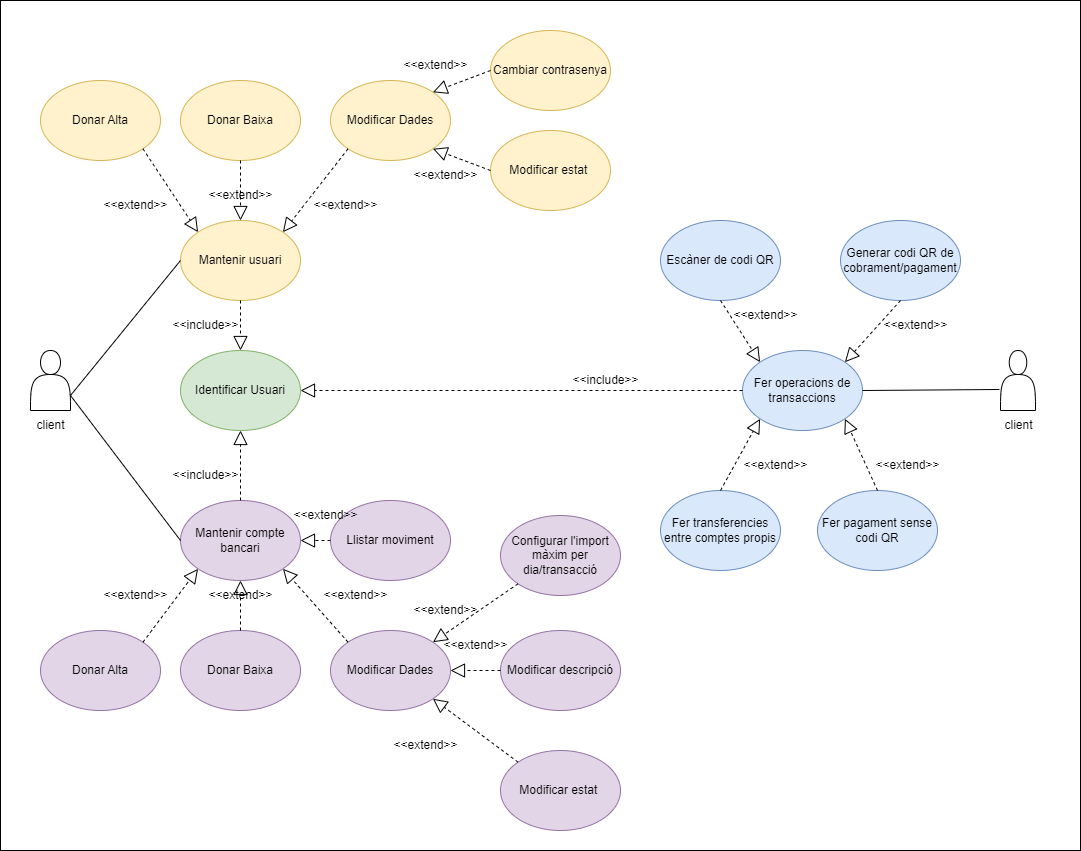
\includegraphics[width=1\textwidth]{imatges/diagrama caso de uso client.png}
    \caption{ Diagrama de Casos d'Ús de Context de Client }
    \label{fig:Diagrama de Casos d'Ús de Context de Client}
\end{figure}

Aquest diagrama de casos d'ús il·lustra les diferents operacions que un \textbf{client} pot realitzar dins del sistema. Encara que hi ha dues instàncies de l'actor client, aquestes representen el mateix actor i es mostren així per a millorar la llegibilitat del gràfic. Cadascuna d'aquestes instàncies està connectada a diversos casos d'ús.

L'actor client pot realitzar operacions relacionades amb la gestió del seu compte d'usuari, incloent-hi donar-se d'alta, donar-se de baixa, modificar les seves dades personals, canviar la contrasenya i modificar l'estat del seu compte. Totes aquestes operacions formen part d'un cas d'ús més general anomenat \textbf{Mantenir usuari}, que centralitza aquestes funcions. Per poder realitzar aquestes accions, el client ha de passar pel procés d'\textbf{Identificar Usuari}, que és un pas previ necessari per garantir la seguretat de les operacions.\\

A més de gestionar el compte d'usuari, el client també pot gestionar el seu compte bancari a través del cas d'ús \textbf{Mantenir compte bancari}, que inclou accions com donar d'alta un compte, donar-lo de baixa, modificar les dades del compte, llistar els moviments bancaris, i configurar l'import màxim per transacció o per dia. Aquestes funcions estan dissenyades per permetre al client controlar i supervisar les seves operacions bancàries dins del sistema.\\

Un altre grup important de casos d'ús està relacionat amb les \textbf{operacions de transaccions}. Aquí, el client pot escanejar codis QR per realitzar pagaments o cobraments, generar codis QR, fer transferències entre els seus propis comptes i realitzar pagaments sense necessitat d'utilitzar un codi QR. Aquestes operacions són essencials per a la funcionalitat de qualsevol sistema que impliqui gestió financera, ja que permeten al client executar transaccions de manera ràpida i segura.\\



\clearpage
\begin{figure}[h]
    \centering
    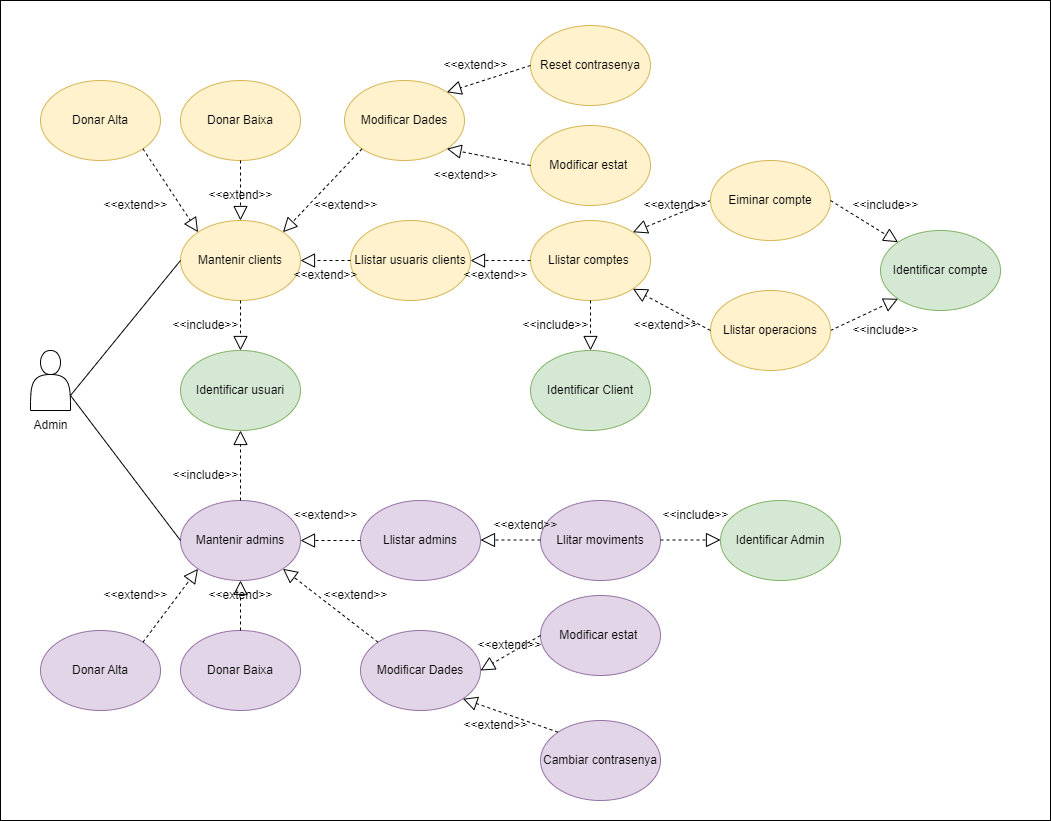
\includegraphics[width=0.9\textwidth]{imatges/diagrama caso de uso admin.png}
    \caption{ Diagrama de Casos d'Ús de Context d'Administrador }
    \label{fig:Diagrama de Casos d'Ús de Context d'Administrador}
\end{figure}


Aquesta segona diagrama d'ús mostra les diferents funcions que un \textbf{administrador} pot dur a terme dins d'un sistema. L'actor principal és l'administrador, qui interactua amb diversos casos d'ús que representen les operacions disponibles. Un dels casos d'ús centrals és \textbf{mantenir clients}, que inclou accions com donar d'alta nous clients, donar de baixa clients existents, modificar les dades dels clients, llistar els usuaris clients, restablir la contrasenya dels clients i modificar l'estat dels clients. Un altre cas d'ús important és \textbf{mantenir admins}, que implica afegir nous administradors, eliminar administradors, modificar les dades dels administradors, llistar els administradors existents i modificar l'estat dels administradors.\\

A més, el diagrama mostra altres casos d'ús relacionats amb la gestió de comptes i operacions. Llistar comptes permet veure la llista de comptes de clients, mentre que eliminar compte s'encarrega d'eliminar un compte de client. Llistar operacions permet revisar les operacions realitzades pels clients, i llistar moviments té una funció similar però aplicada als comptes o admins. També hi ha casos d'ús que fan referència a la identificació d'usuaris, comptes, clients i admins, mostrant la interrelació entre aquestes operacions i la necessitat d'autenticació o identificació per dur-les a terme.



\clearpage
\begin{figure}[h]
    \centering
    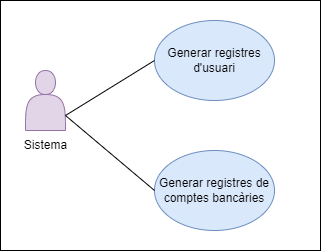
\includegraphics[width=0.6\textwidth]{imatges/logs.png}
    \caption{ Diagrama de Casos d'Ús de Context del sistema }
    \label{fig:Diagrama de Casos d'Ús de Context del sistema}
\end{figure}


Adicionalment, el sistema disposa de la funció de generar logs per a cada operació. Això significa que, fins i tot en cas d'eliminació d'un usuari o un compte, l'historial associat es manté sempre guardat. Aquest enfocament assegura la conservació de dades importants per a possibles auditories o revisió posterior, garantint la traçabilitat i la seguretat del sistema.

\clearpage
\section{diagrama de base de dades}
\label{sec: diagrama de base de dades}


\begin{figure}[h]
    \centering
    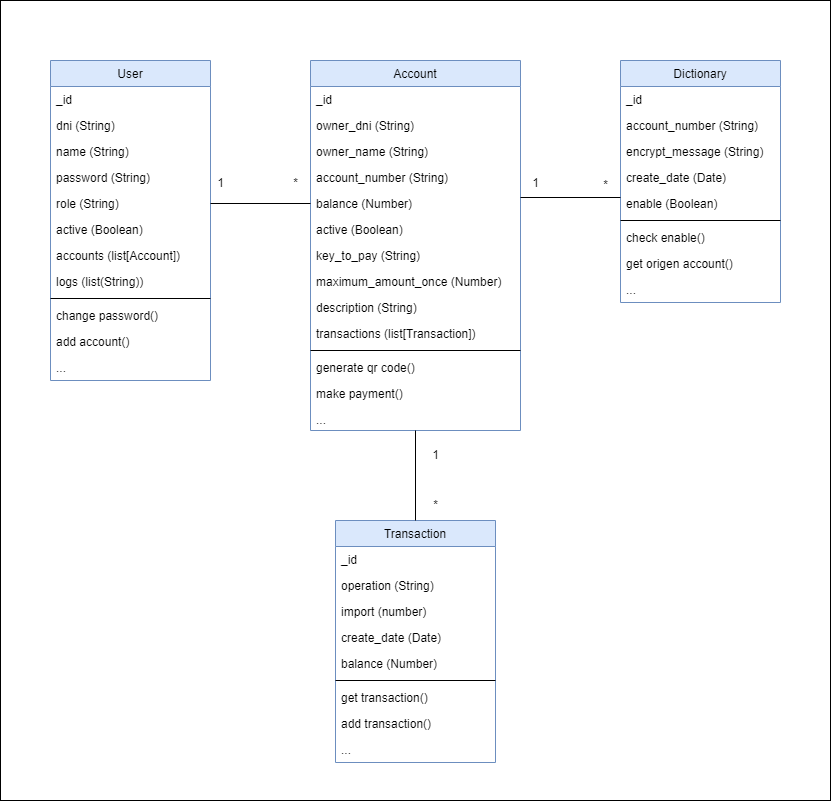
\includegraphics[width=1\textwidth]{imatges/diagrama base dades.png}
    \caption{ Diagrama de base de dades }
    \label{fig: Diagrama de base de dades}
\end{figure}

El diagrama representa un model de dades que inclou quatre entitats principals: User, Account, Transaction i Dictionary. Aquestes entitats estan interrelacionades per gestionar informació d'usuaris, comptes, transaccions i altres dades associades.

\subsection{User}
\label{subsec: User}


L'entitat \textbf{User} defineix els usuaris del sistema amb atributs bàsics com el DNI, el nom, la contrasenya, el rol dins del sistema (administrador o client), així com altres camps com l'estat actiu, la llista de comptes associats i els registres d'activitat (logs). Aquesta entitat ofereix funcionalitats per canviar la contrasenya, afegir comptes nous i altres operacions relacionades amb l'usuari.\\

Aquesta entitat conté les dades obligatòries que cada usuari ha de tenir:

\begin{itemize}
    \item \textbf{\_id} (Object\_id) [Clau primària]: Generat automàticament per MongoDB.
    \item \textbf{dni} (String) [NOT NULL]: Emmagatzema el número d'identificació de l'usuari, no repetible.
    \item \textbf{name} (String) [NOT NULL]: Emmagatzema el nom de l'usuari.
    \item \textbf{password} (String) [NOT NULL]: Emmagatzema la contrasenya de l'usuari, que s'encripta abans d'inserir-la.
    \item \textbf{role} (String) [NOT NULL]: Emmagatzema el rol de l'usuari, que pot ser admin o client.
    \item \textbf{active} (Boolean) [DEFAULT: "true"]: Indica si l'usuari està disponible per fer operacions de transacció.
    \item \textbf{accounts} (Account List) [DEFAULT: []]: Emmagatzema tots els ID de comptes que pertanyen a l'usuari.
    \item \textbf{logs} (String List) [DEFAULT: []]: Emmagatzema els moviments de l'usuari.
\end{itemize}


\subsection{Account}
\label{subsec: Account}


L'entitat \textbf{Account} representa els comptes bancaris associats als usuaris. Cada compte té atributs per identificar el propietari, el saldo disponible, una clau per generar codis QR de pagament, límits de transacció, i una descripció del compte. Els comptes poden generar codis QR per facilitar pagaments o cobraments i tenen associades llistes de transaccions.\\

Cada vegada que es genera un codi QR de pagament, la clau s'actualitza i es guarda la informació necessària en la \textbf{Dictionary}. Quan un client escaneja el codi QR, a partir de la Dictionary es pot identificar el propietari i obtenir la clau per desxifrar el missatge.\\

Aquesta entitat conté les dades obligatòries que cada compte ha de tenir:

\begin{itemize}
    \item \textbf{\_id} (Object\_id) [Clau primària]: Generat automàticament per MongoDB.
    \item \textbf{owner\_dni} (String) [NOT NULL]: Emmagatzema el DNI del propietari del compte.
    \item \textbf{owner\_name} (String) [NOT NULL]: Emmagatzema el nom del propietari del compte.
    \item \textbf{account\_number} (String) [NOT NULL]: Emmagatzema el número de compte, que ha de ser únic.
    \item \textbf{balance} (Number) [NOT NULL]: Emmagatzema el saldo disponible en el compte.
    \item \textbf{active} (Boolean) [DEFAULT: "true"]: Indica si el compte està actiu i pot realitzar transaccions.
    \item \textbf{key\_to\_pay} (String) [NOT NULL]: Emmagatzema una clau per generar codis QR de pagament.
    \item \textbf{maximum\_amount\_once} (Number) [DEFAULT: 0]: Indica la quantitat màxima que es pot pagar en una sola transacció.
    \item \textbf{description} (String) [OPTIONAL]: Conté una descripció addicional del compte.
    \item \textbf{transactions} (Transaction List) [DEFAULT: []]: Emmagatzema la llista de transaccions associades al compte.
\end{itemize}




\subsection{Dictionary}
\label{subsec: Dictionary}

L'entitat \textbf{Dictionary} emmagatzema informació complementària relacionada amb els comptes i les transaccions. Aquesta entitat es fa servir per guardar dades com missatges encriptats, dates de creació, i estats d'activació, permetent verificar i processar correctament les operacions financeres dins del sistema.\\


\begin{figure}[h]
    \centering
    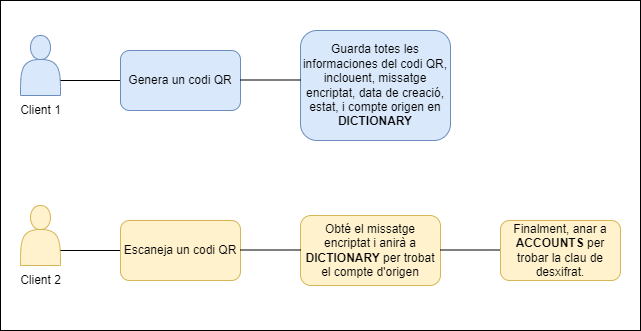
\includegraphics[width=0.7\textwidth]{imatges/dictionary.png}
    \caption{ Ús de Dictionary }
    \label{fig: Ús de Dictionary}
\end{figure}


Aquesta entitat conté les dades obligatòries que cada entrada ha de tenir:

\begin{itemize}
    \item \textbf{\_id} (Object\_id) [Clau primària]: Generat automàticament per MongoDB.
    \item \textbf{account\_number} (String) [NOT NULL]: Emmagatzema el número de compte associat.
    \item \textbf{encrypt\_message} (String) [NOT NULL]: Conté el missatge encriptat relacionat amb la transacció.
    \item \textbf{create\_date} (Date) [NOT NULL]: Indica la data de creació de l'entrada al diccionari.
    \item \textbf{enable} (Boolean) [DEFAULT: "true"]: Indica si l'entrada està activa i disponible per ser utilitzada.
\end{itemize}



\subsection{Transaction}
\label{subsec: Transaction}


L'entitat \textbf{Transaction} descriu les operacions financeres realitzades en un compte. Aquesta entitat emmagatzema informació detallada sobre cada transacció, com ara el tipus d'operació, l'import, i el saldo resultant. Cada transacció genera dues instàncies: una per al compte d'origen (qui paga) i una altra per al compte de destí (qui cobra). Aquest diagrama reflecteix com les entitats es connecten per permetre la gestió d'usuaris, comptes i transaccions dins del sistema.\\

Aquesta entitat conté les dades obligatòries que cada transacció ha de tenir:

\begin{itemize}
    \item \textbf{\_id} (Object\_id) [Clau primària]: Generat automàticament per MongoDB.
    \item \textbf{operation} (String) [NOT NULL]: Indica el tipus d'operació realitzada (per exemple, "pagament" o "cobrament").
    \item \textbf{amount} (Number) [NOT NULL]: Emmagatzema l'import de la transacció.
    \item \textbf{create\_date} (Date) [NOT NULL]: Indica la data de creació de la transacció.
    \item \textbf{balance} (Number) [NOT NULL]: Reflecteix el saldo resultant en el compte després de la transacció.
    \item \textbf{origin\_account} (String) [NOT NULL]: Emmagatzema el número de compte d'origen de la transacció.
    \item \textbf{destination\_account} (String) [NOT NULL]: Emmagatzema el número de compte de destí de la transacció.
\end{itemize}


\section{ Interfícies d'usuari }
\label{ sec: Interfícies d'usuari }


El disseny de les interfícies d'usuari ha estat una prioritat abans d'endinsar-nos en el desenvolupament del front-end. Aquestes interfícies proporcionen una visió preliminar de l'aspecte i la sensació que tindrà l'aplicació. Les figures següents mostren els dissenys de les interfícies d'usuari. \\

Dissenyar tots els possibles estats de l'aplicació en un temps tan limitat és inviable. No obstant això, atès que l'aplicació principal i la dels usuaris comparteixen gran part de la seva interfície, només s'han dissenyat les vistes principals. En desenvolupar l'aplicació de l'usuari, la majoria dels components s'han reutilitzat, modificant-ne el comportament segons les necessitats, ja que les interaccions dels usuaris són limitades.\\

És important destacar que algunes vistes no corresponen exactament a com són a l'aplicació final, principalment perquè s'han modificat o afegit funcionalitats segons les necessitats durant el desenvolupament.\\


\subsection{Client}
\label{subsec: Client}

\begin{figure}[h]
    \centering
    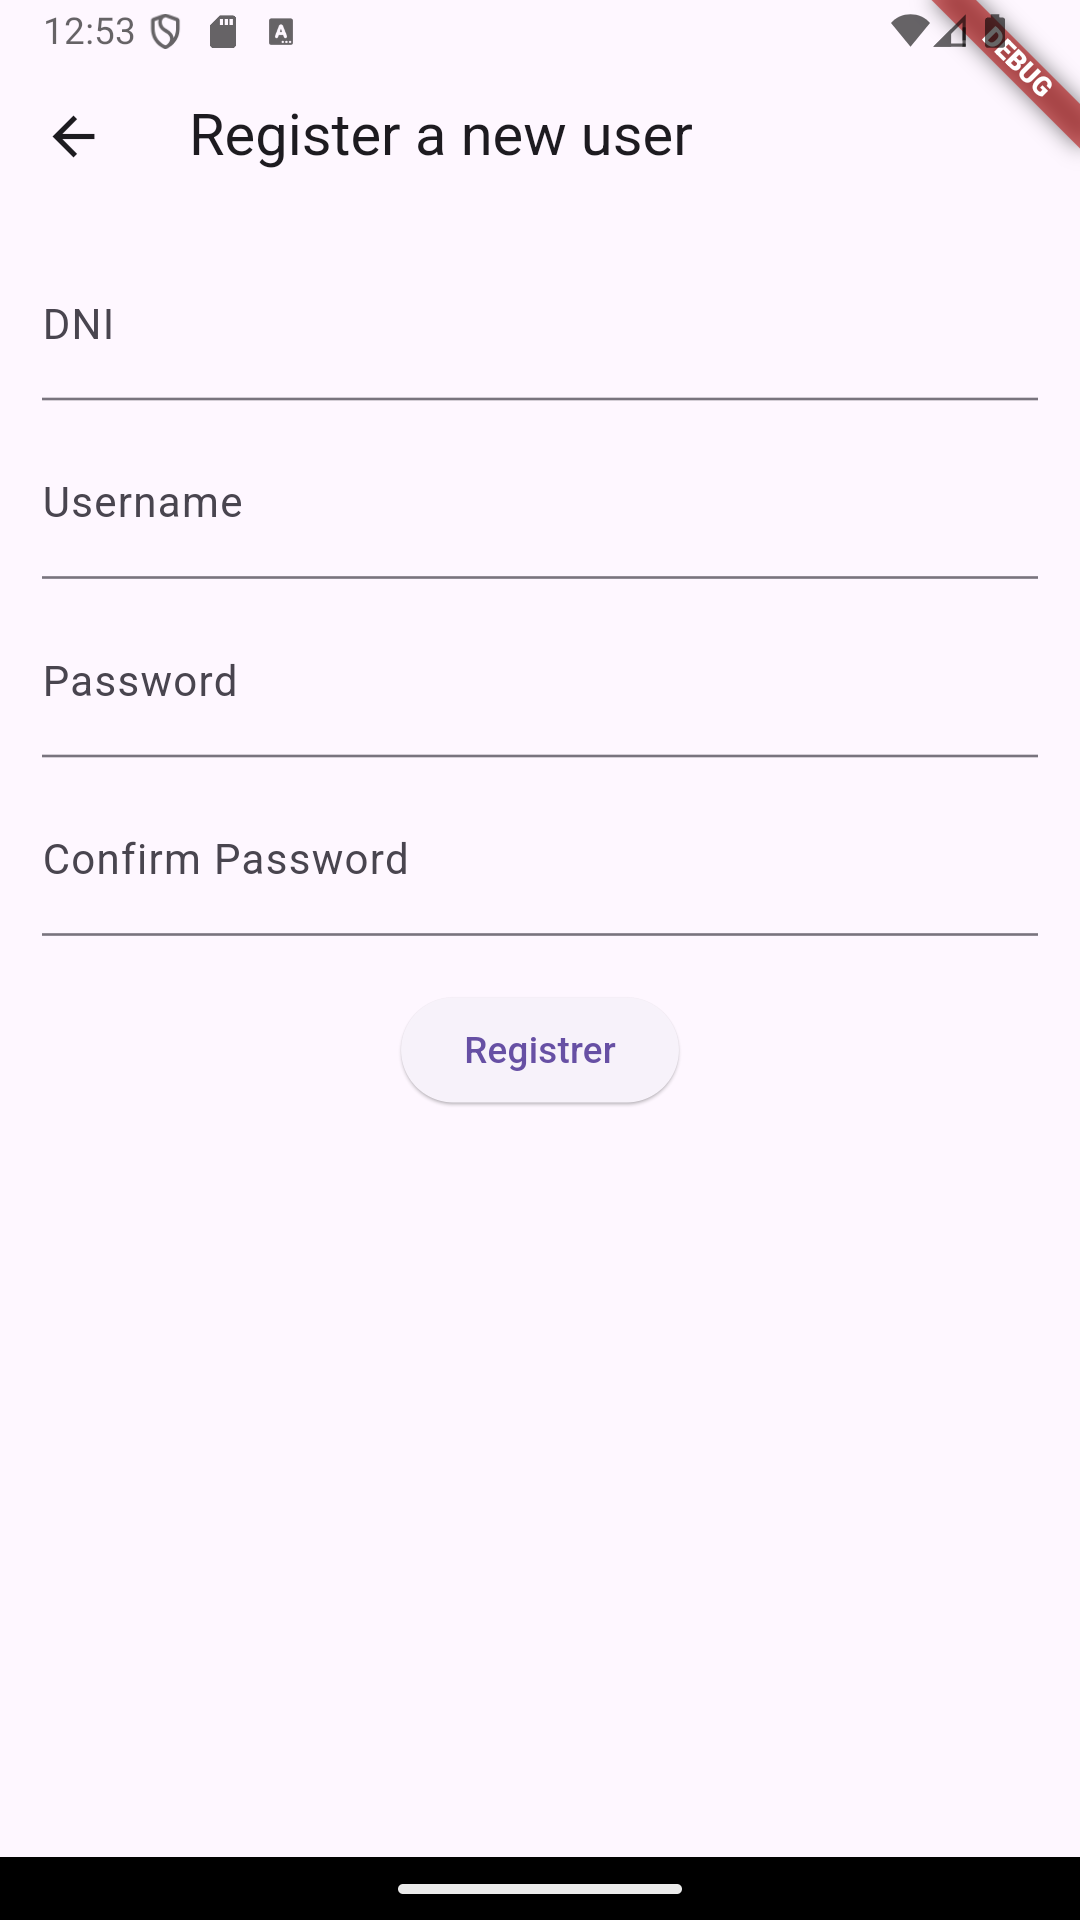
\includegraphics[width=0.3\textwidth]{imatges/registerUser.png}
    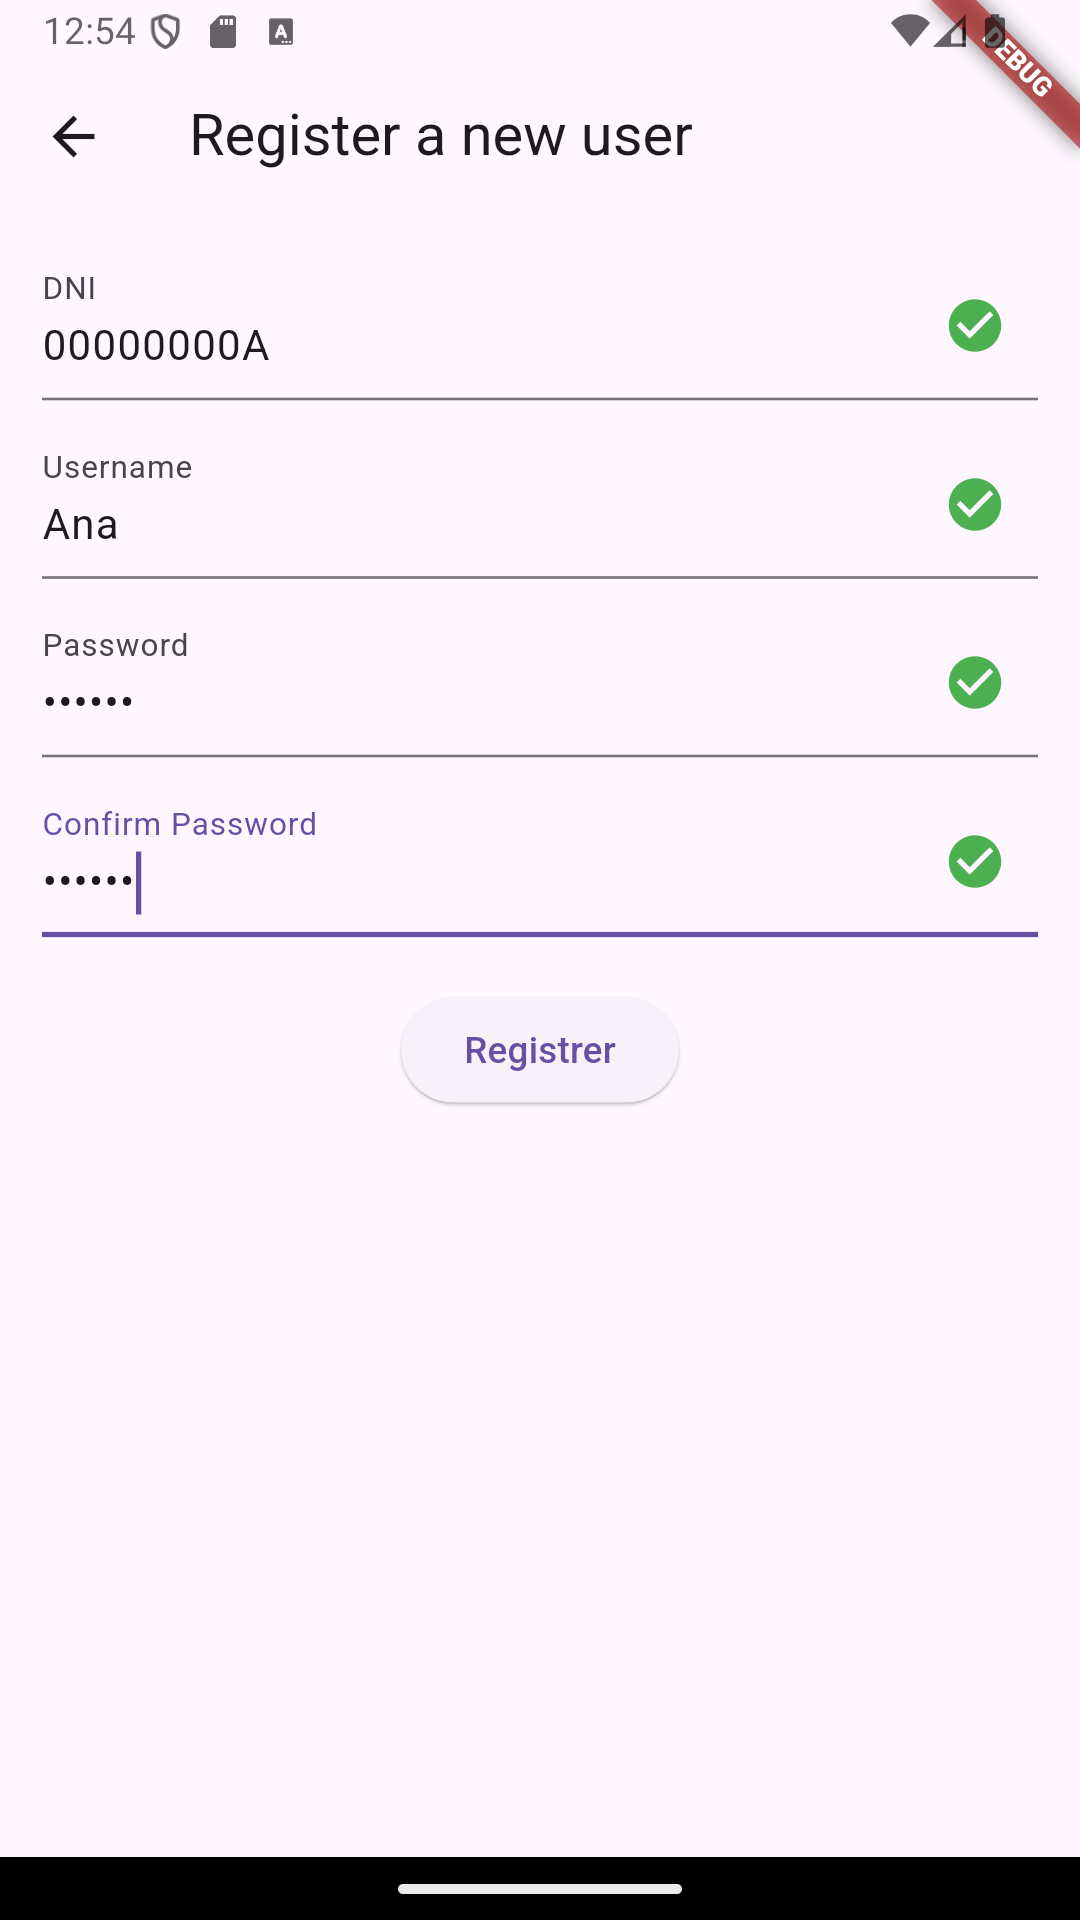
\includegraphics[width=0.3\textwidth]{imatges/registerUserWithvalues.png}
    \caption{ registrar nou usuari}
    \label{fig: registrar nou usuari}
\end{figure}


\begin{figure}[h]
    \centering
    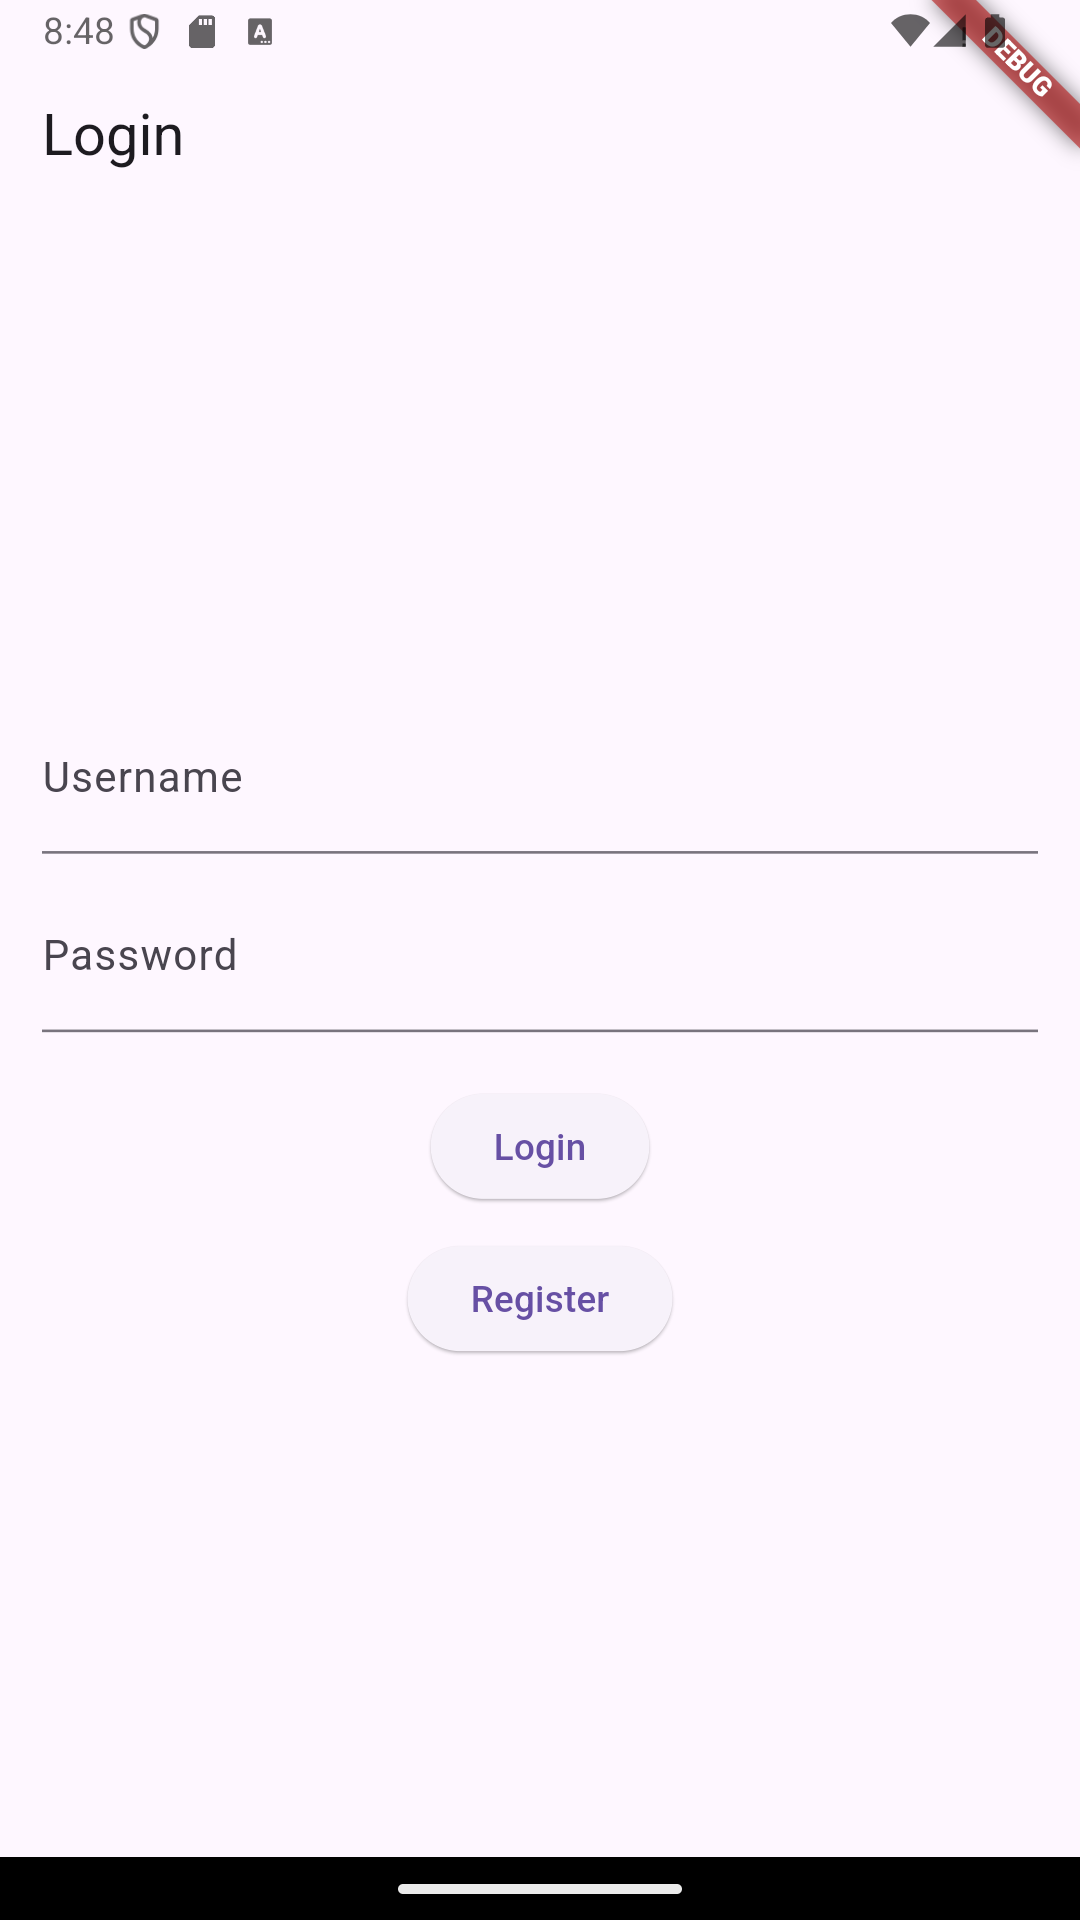
\includegraphics[width=0.3\textwidth]{imatges/login.png}
    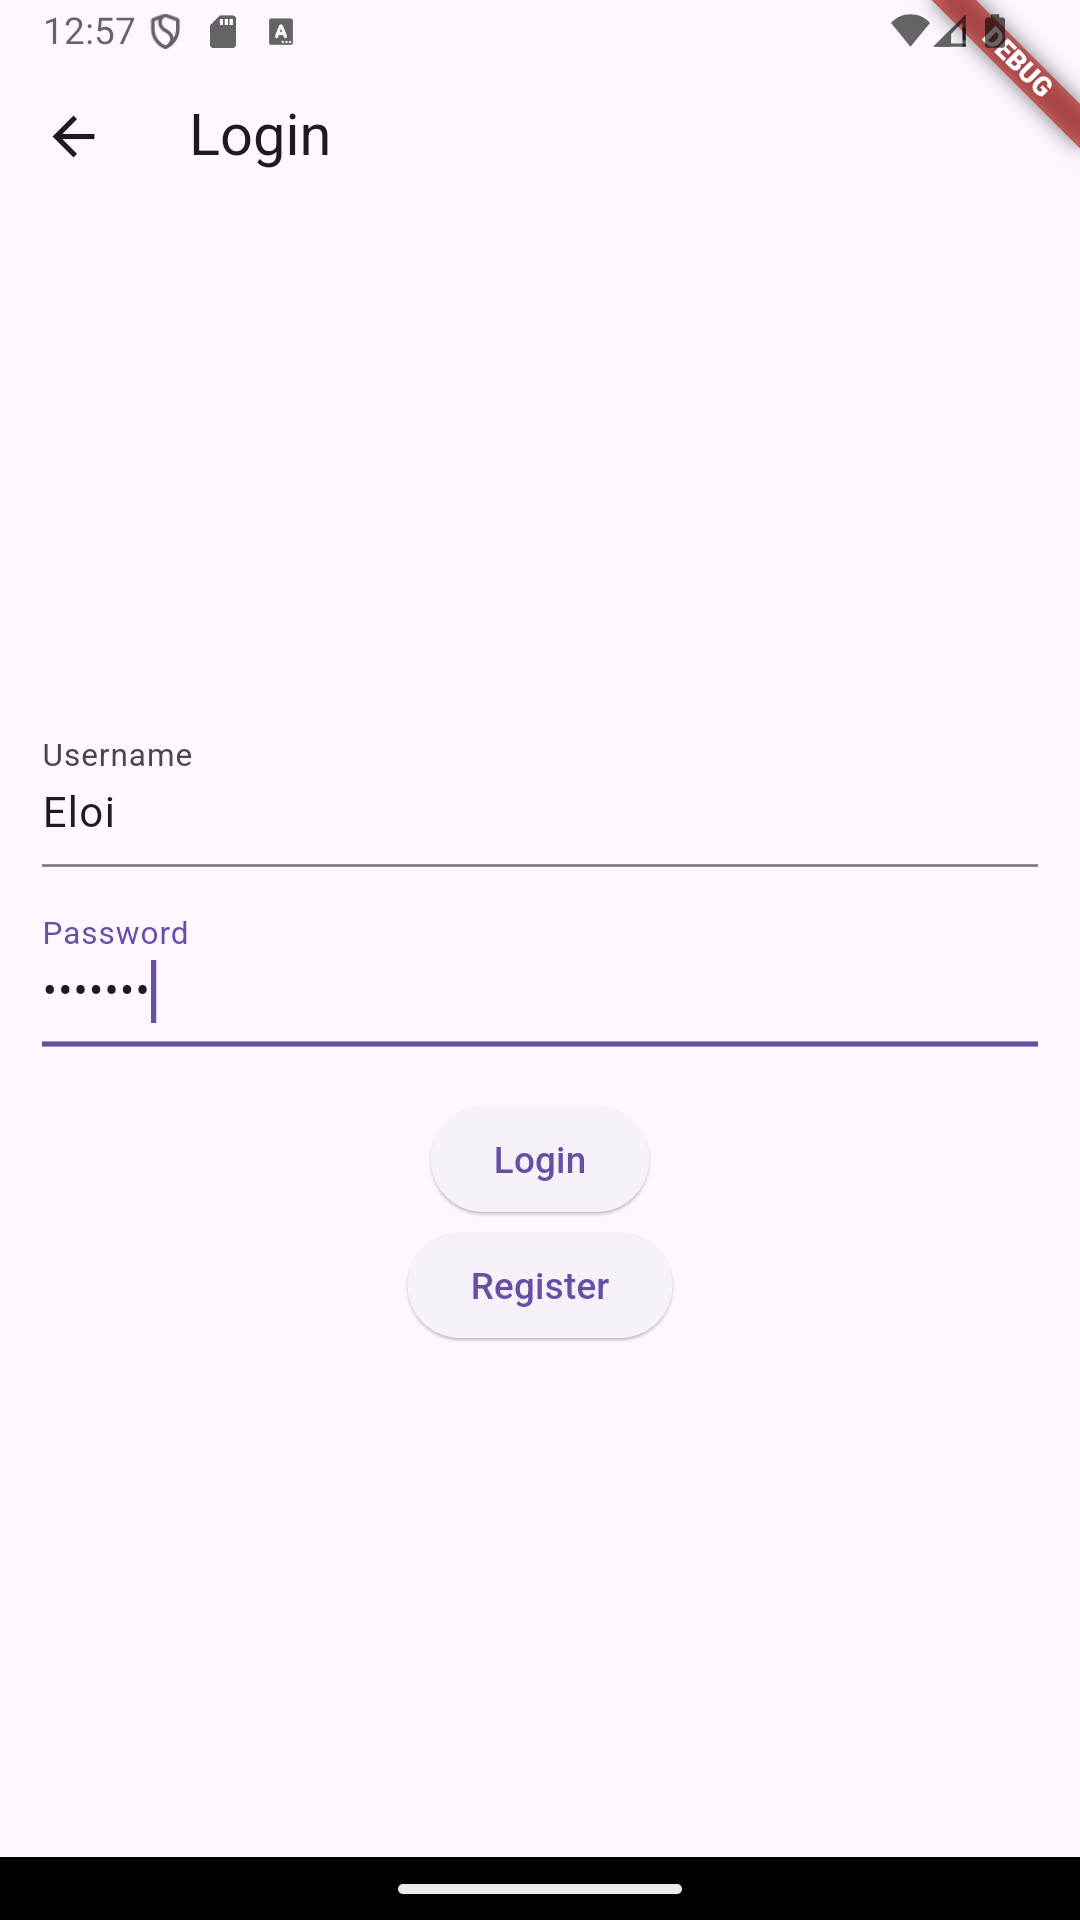
\includegraphics[width=0.3\textwidth]{imatges/loginWithValue.png}
    \caption{ Pàgina de login - client}
    \label{fig: Pàgina de login - client}
\end{figure}



\begin{figure}[h]
    \centering
    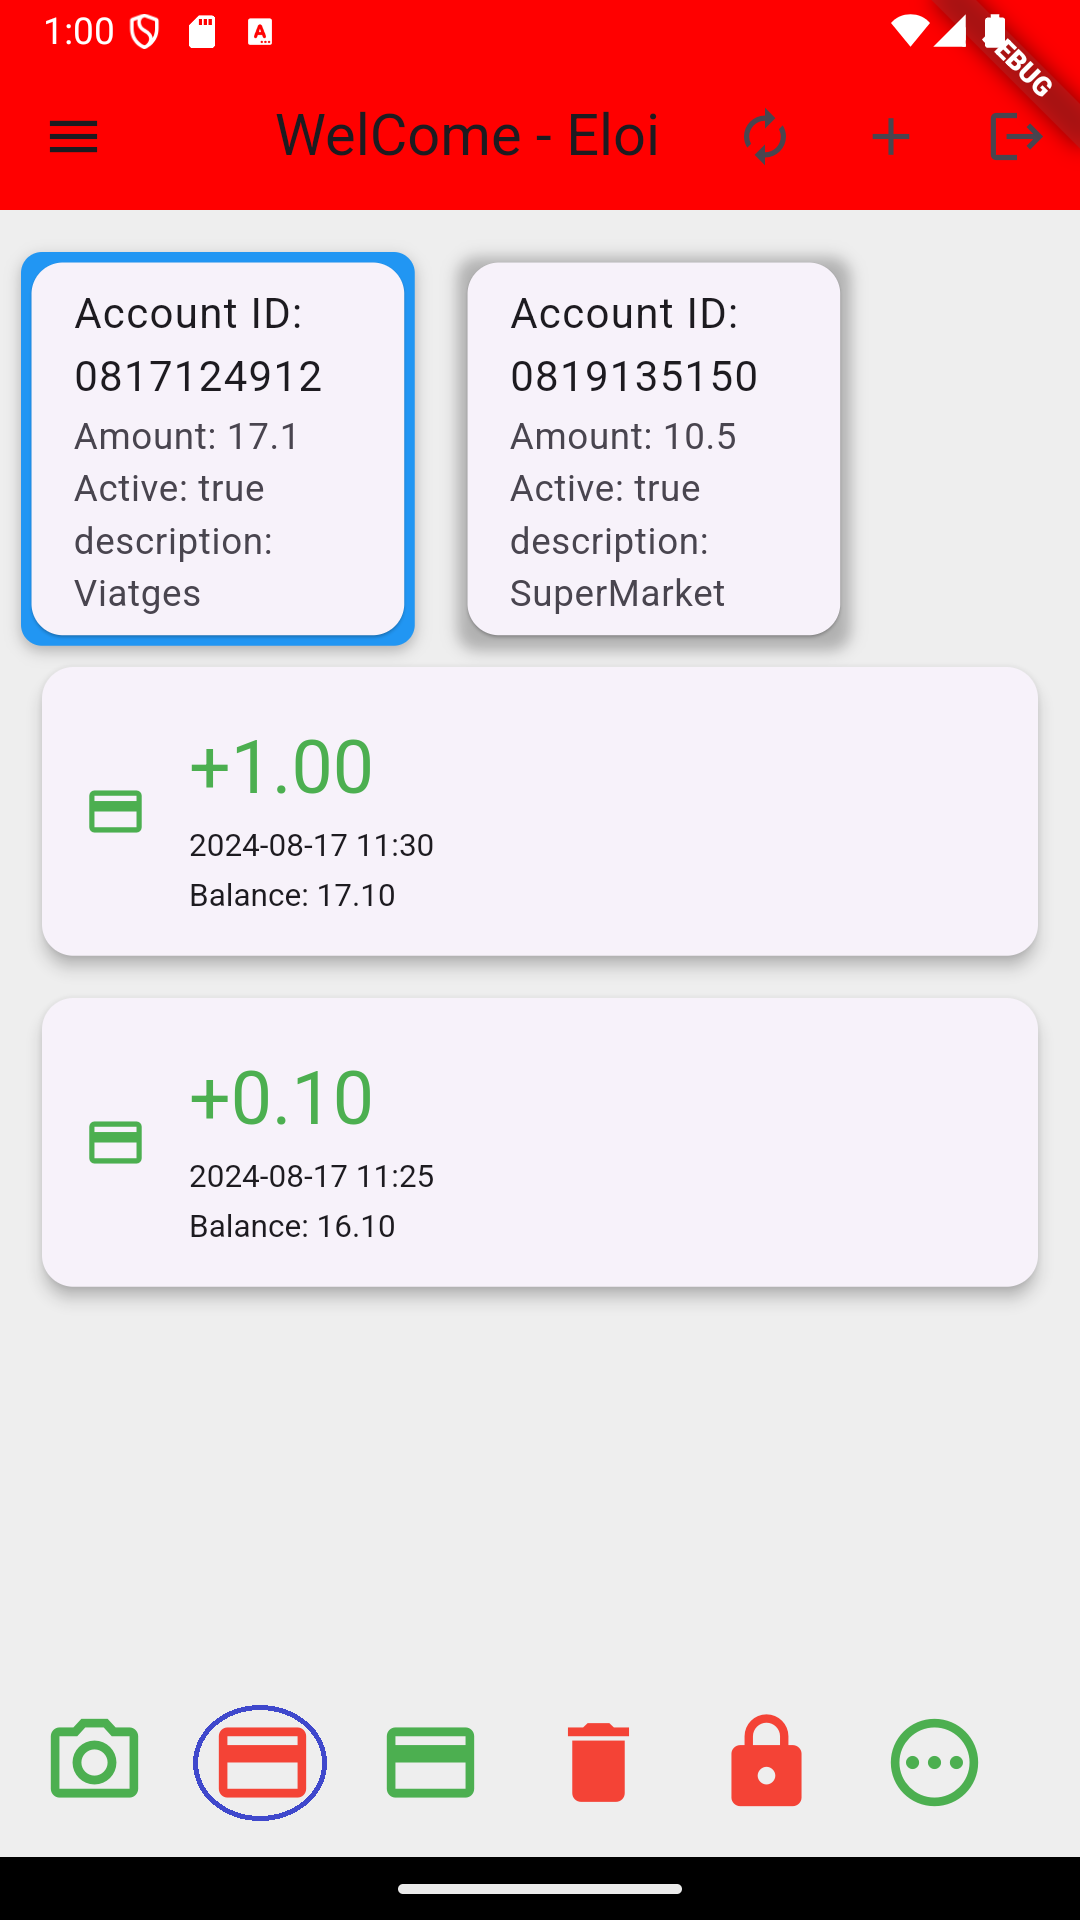
\includegraphics[width=0.3\textwidth]{imatges/mainPage2.png}
    
\includegraphics[width=0.3\textwidth]{imatges/paymentPage.png}
    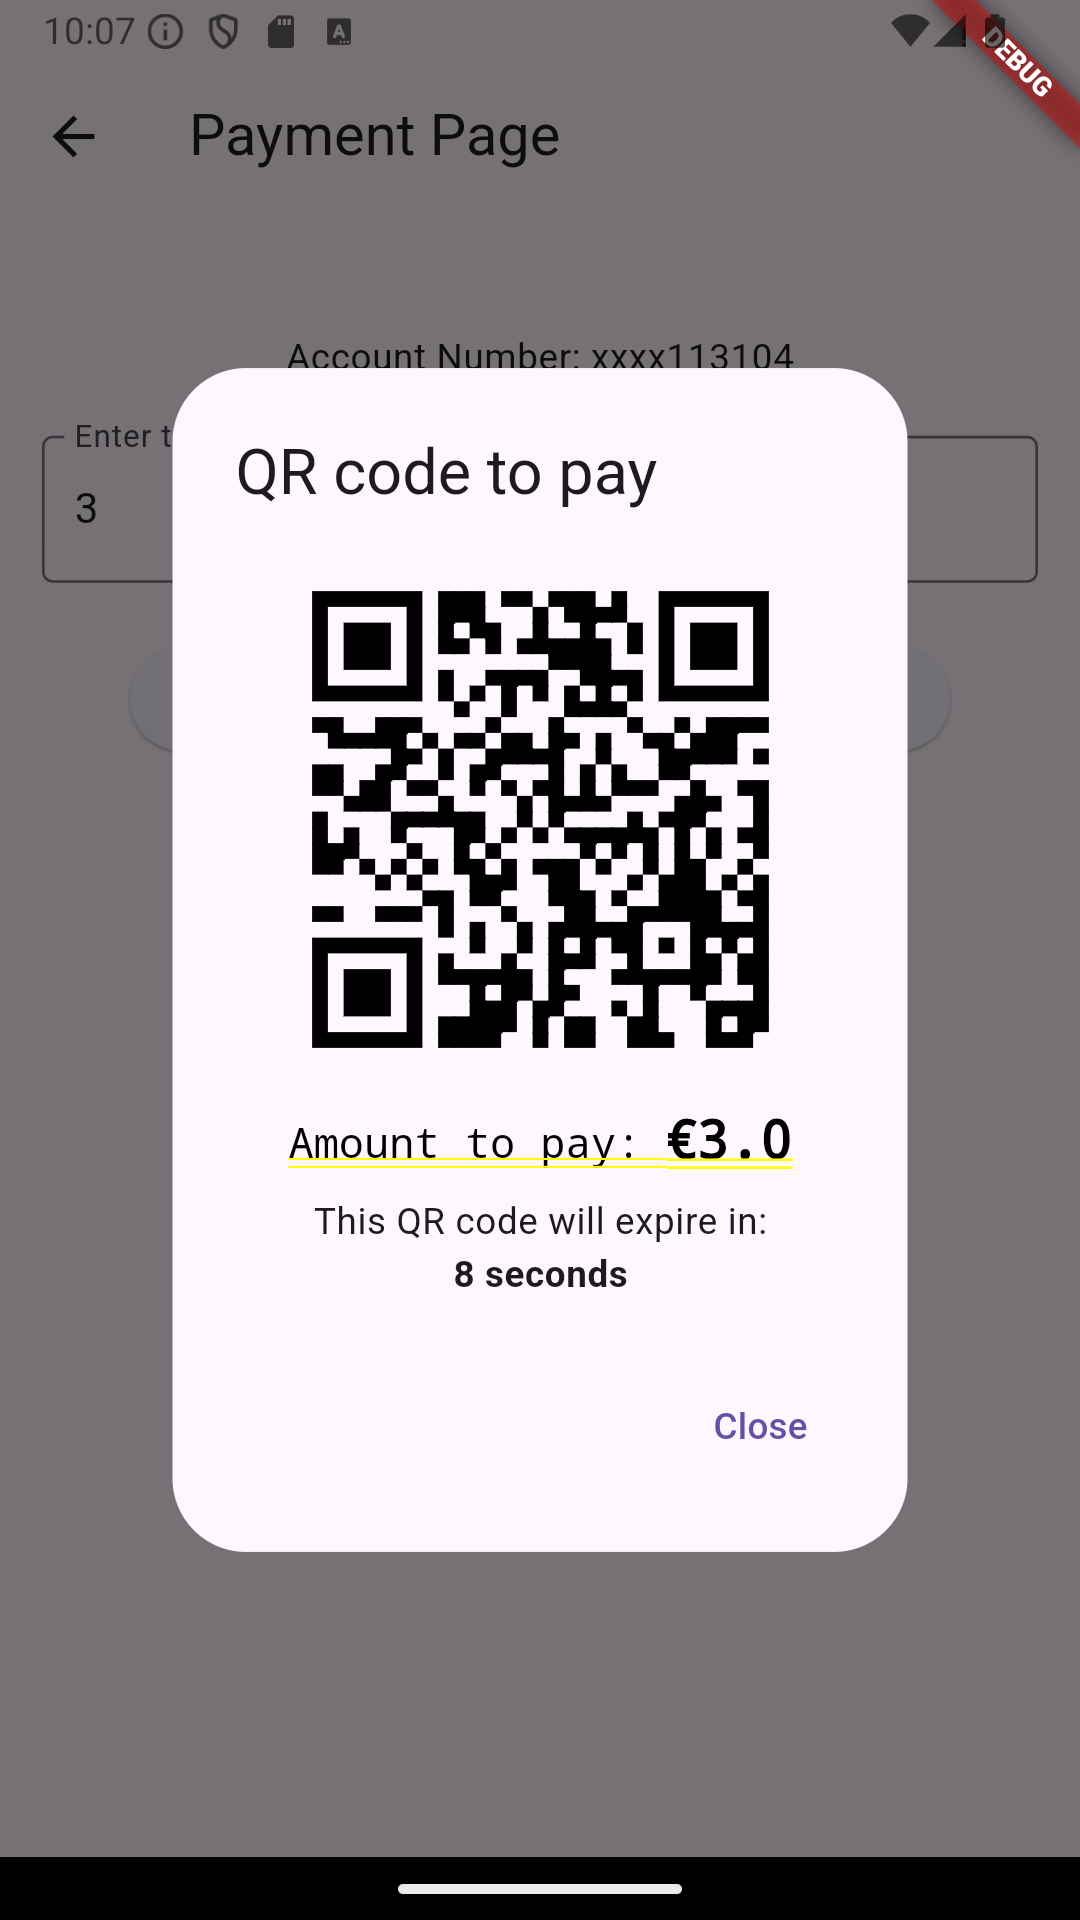
\includegraphics[width=0.3\textwidth]{imatges/paymentPageWithValue.png}
    \caption{ Pàgina per generar codi QR de pagament}
    \label{fig: Pàgina per generar codi QR de pagament}
\end{figure}

\begin{figure}[h]
    \centering
    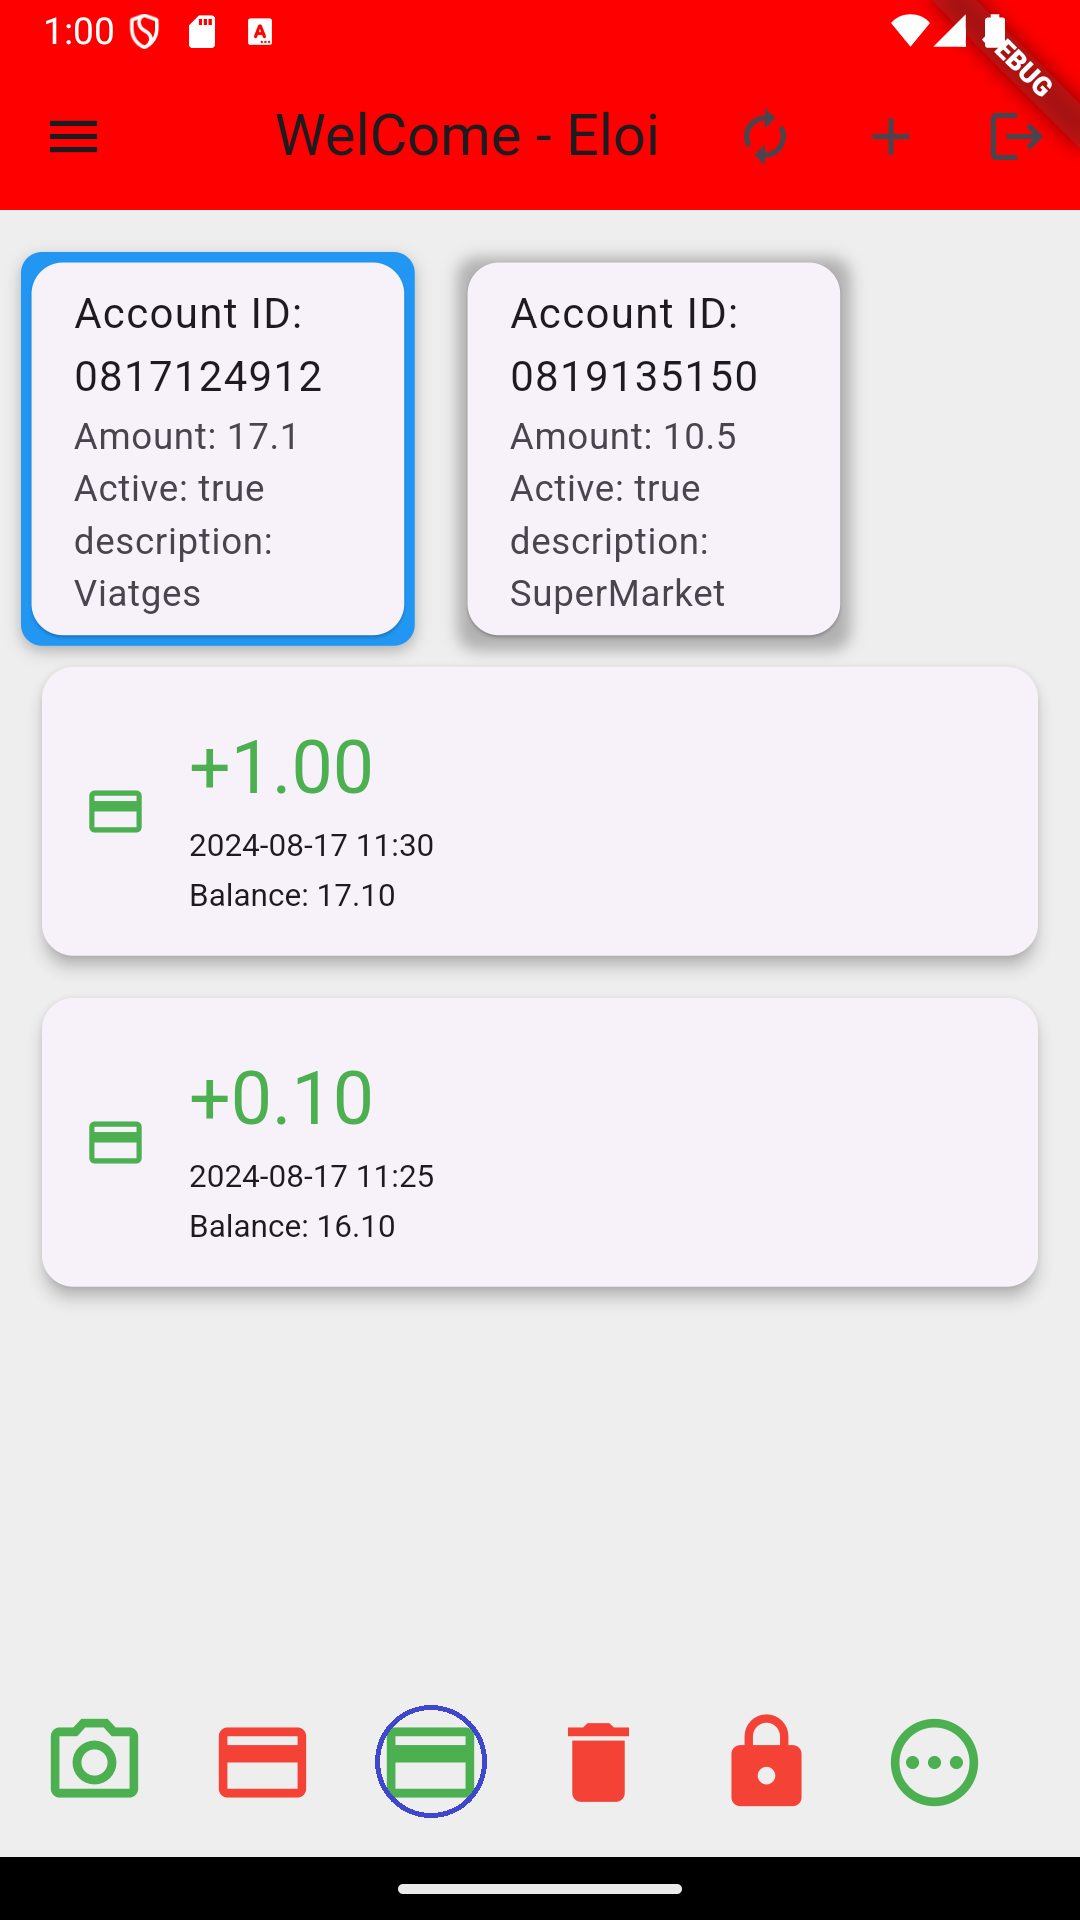
\includegraphics[width=0.3\textwidth]{imatges/mainPage3.png}
    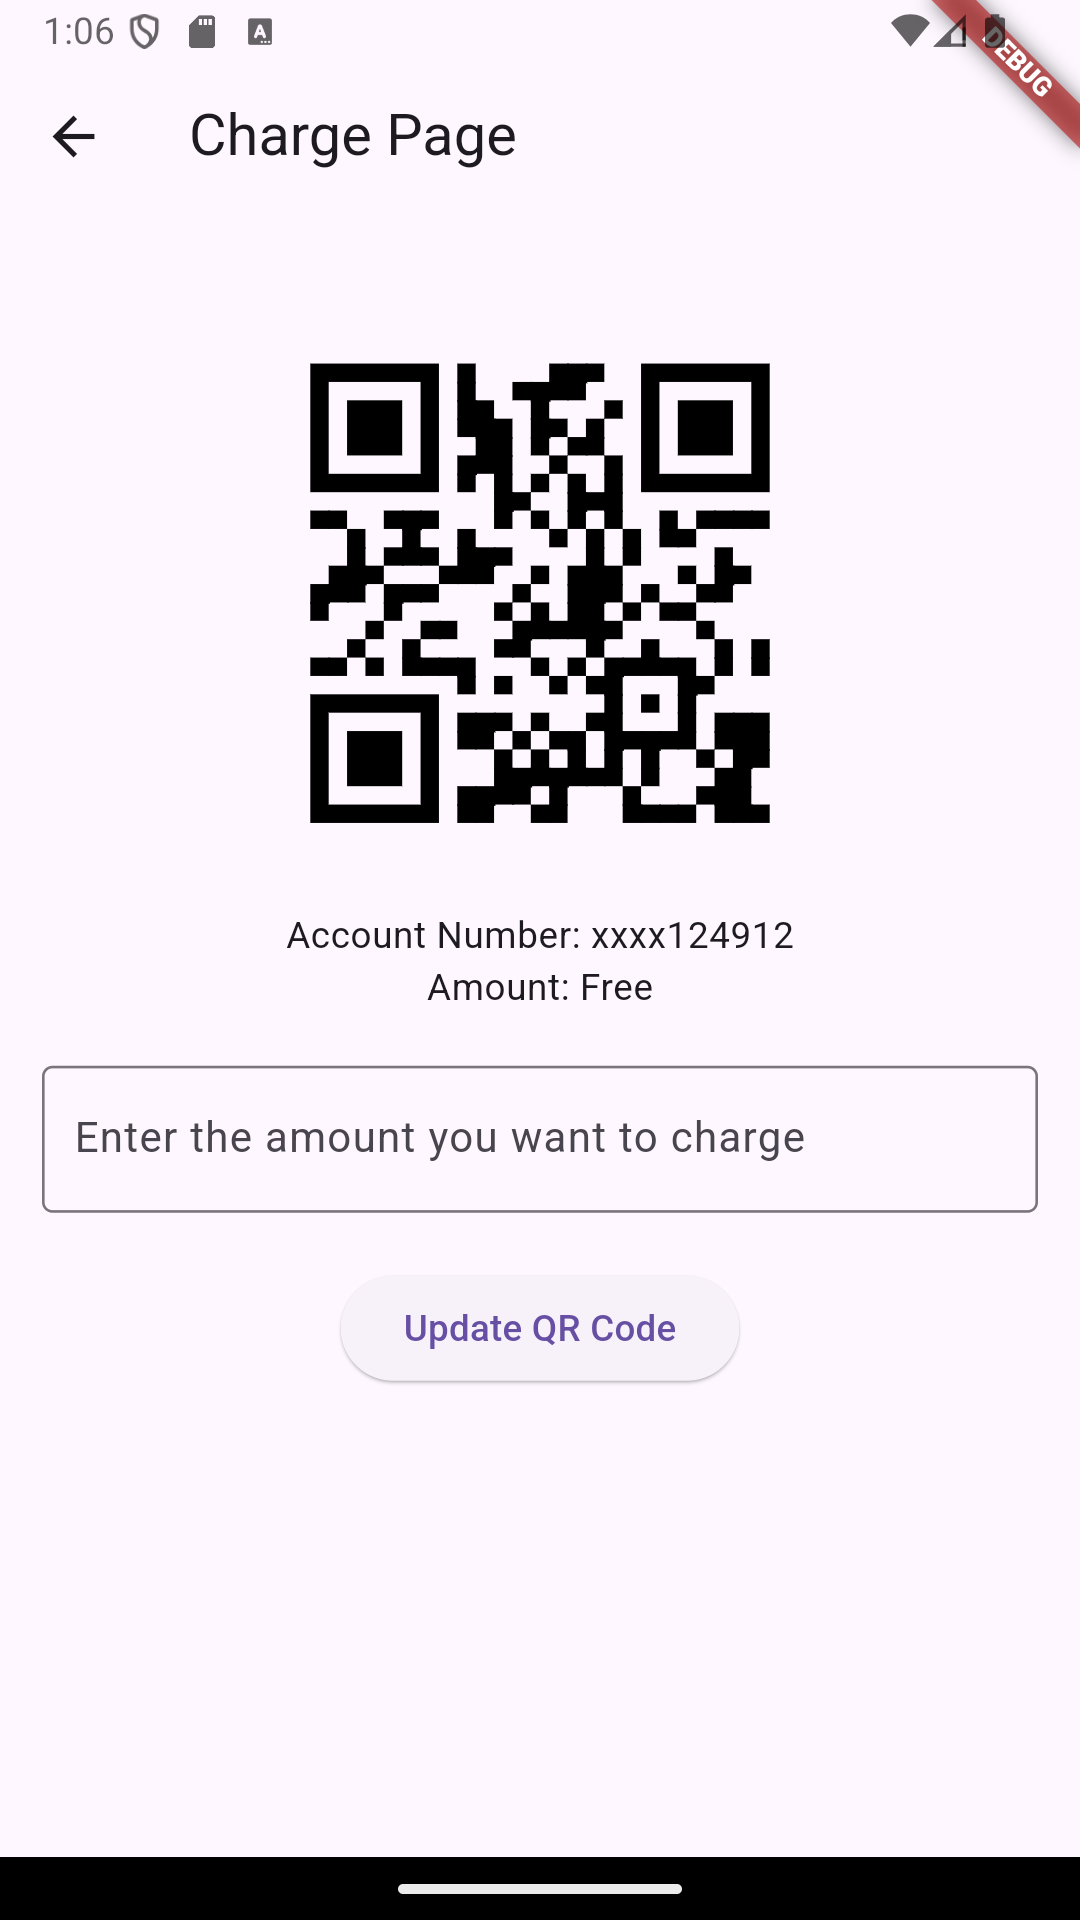
\includegraphics[width=0.3\textwidth]{imatges/chargePage.png}
    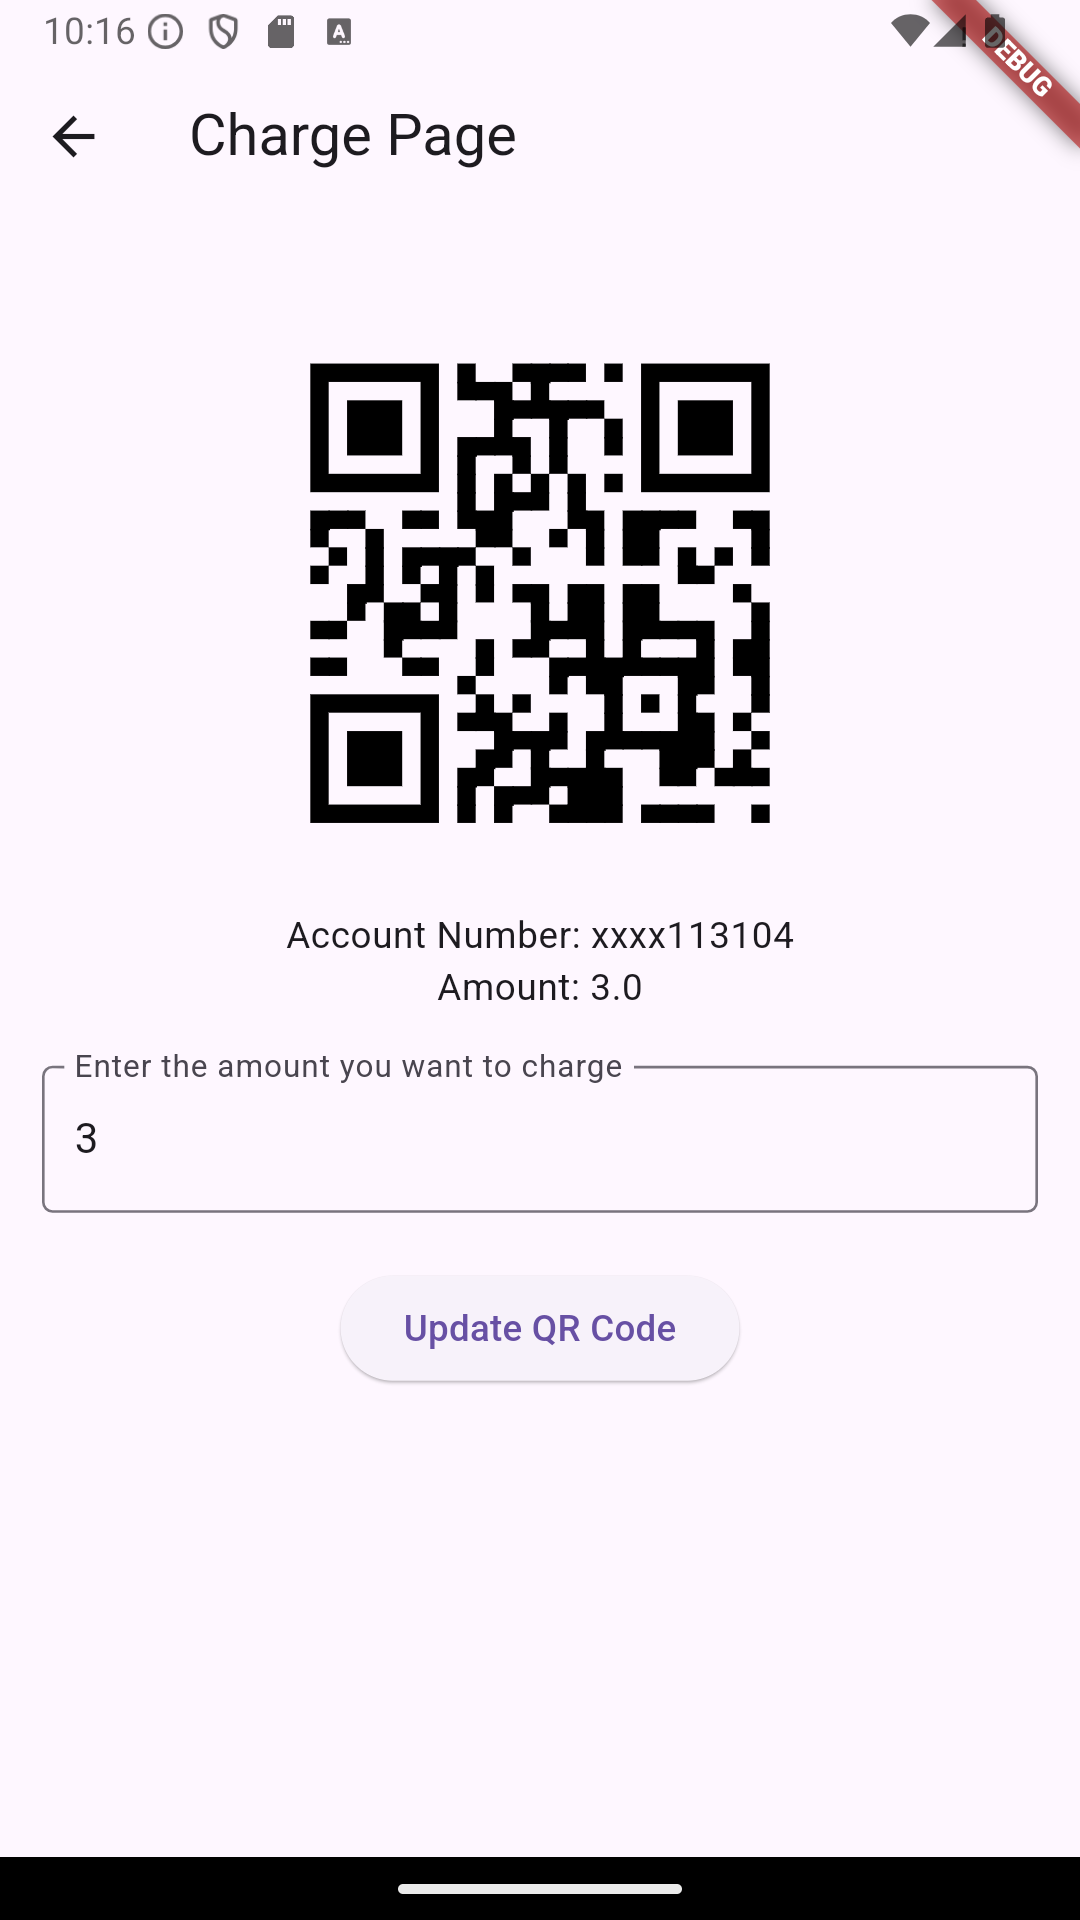
\includegraphics[width=0.3\textwidth]{imatges/chargePageWithValue.png}
    \caption{ Pàgina per generar codi QR de cobrament}
    \label{fig: Pàgina per generar codi QR de cobrament}
\end{figure}

\begin{figure}[h]
    \centering
    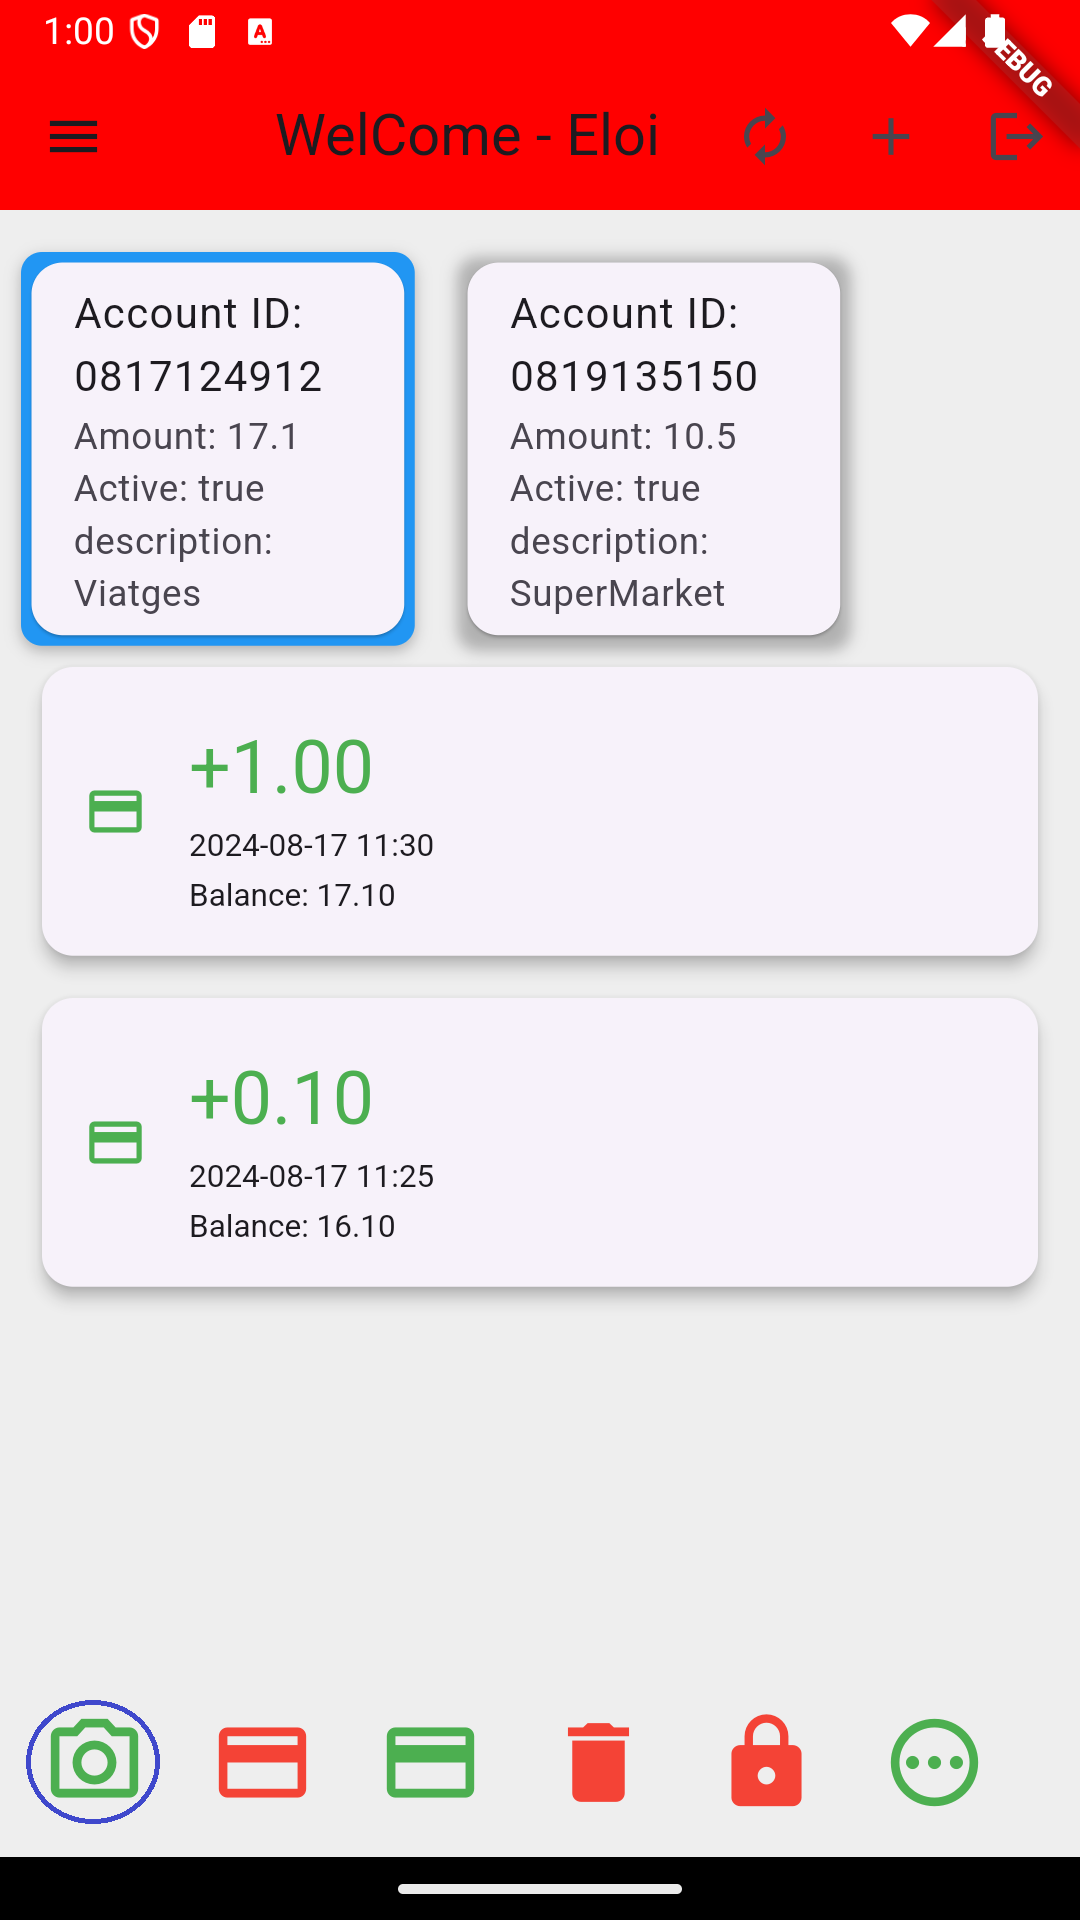
\includegraphics[width=0.3\textwidth]{imatges/mainPage1.png}
    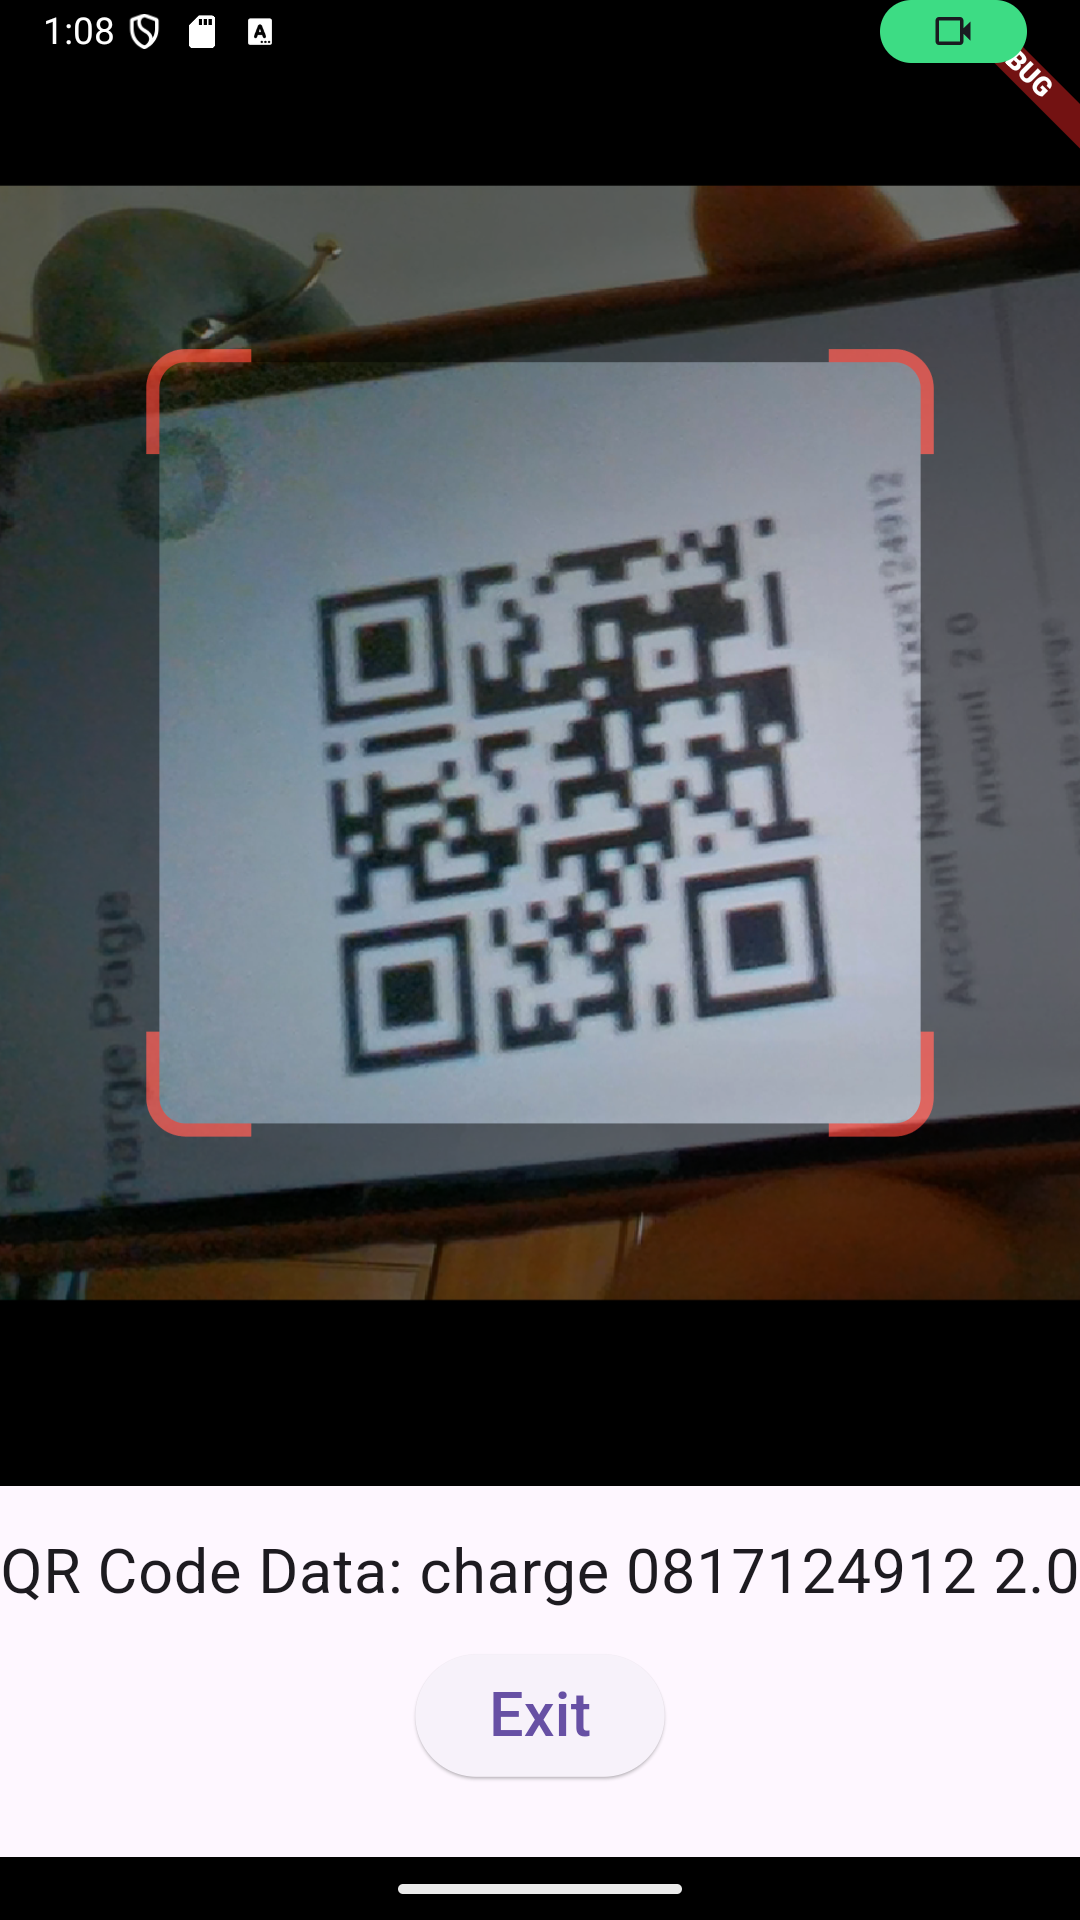
\includegraphics[width=0.3\textwidth]{imatges/scanQR.png}
    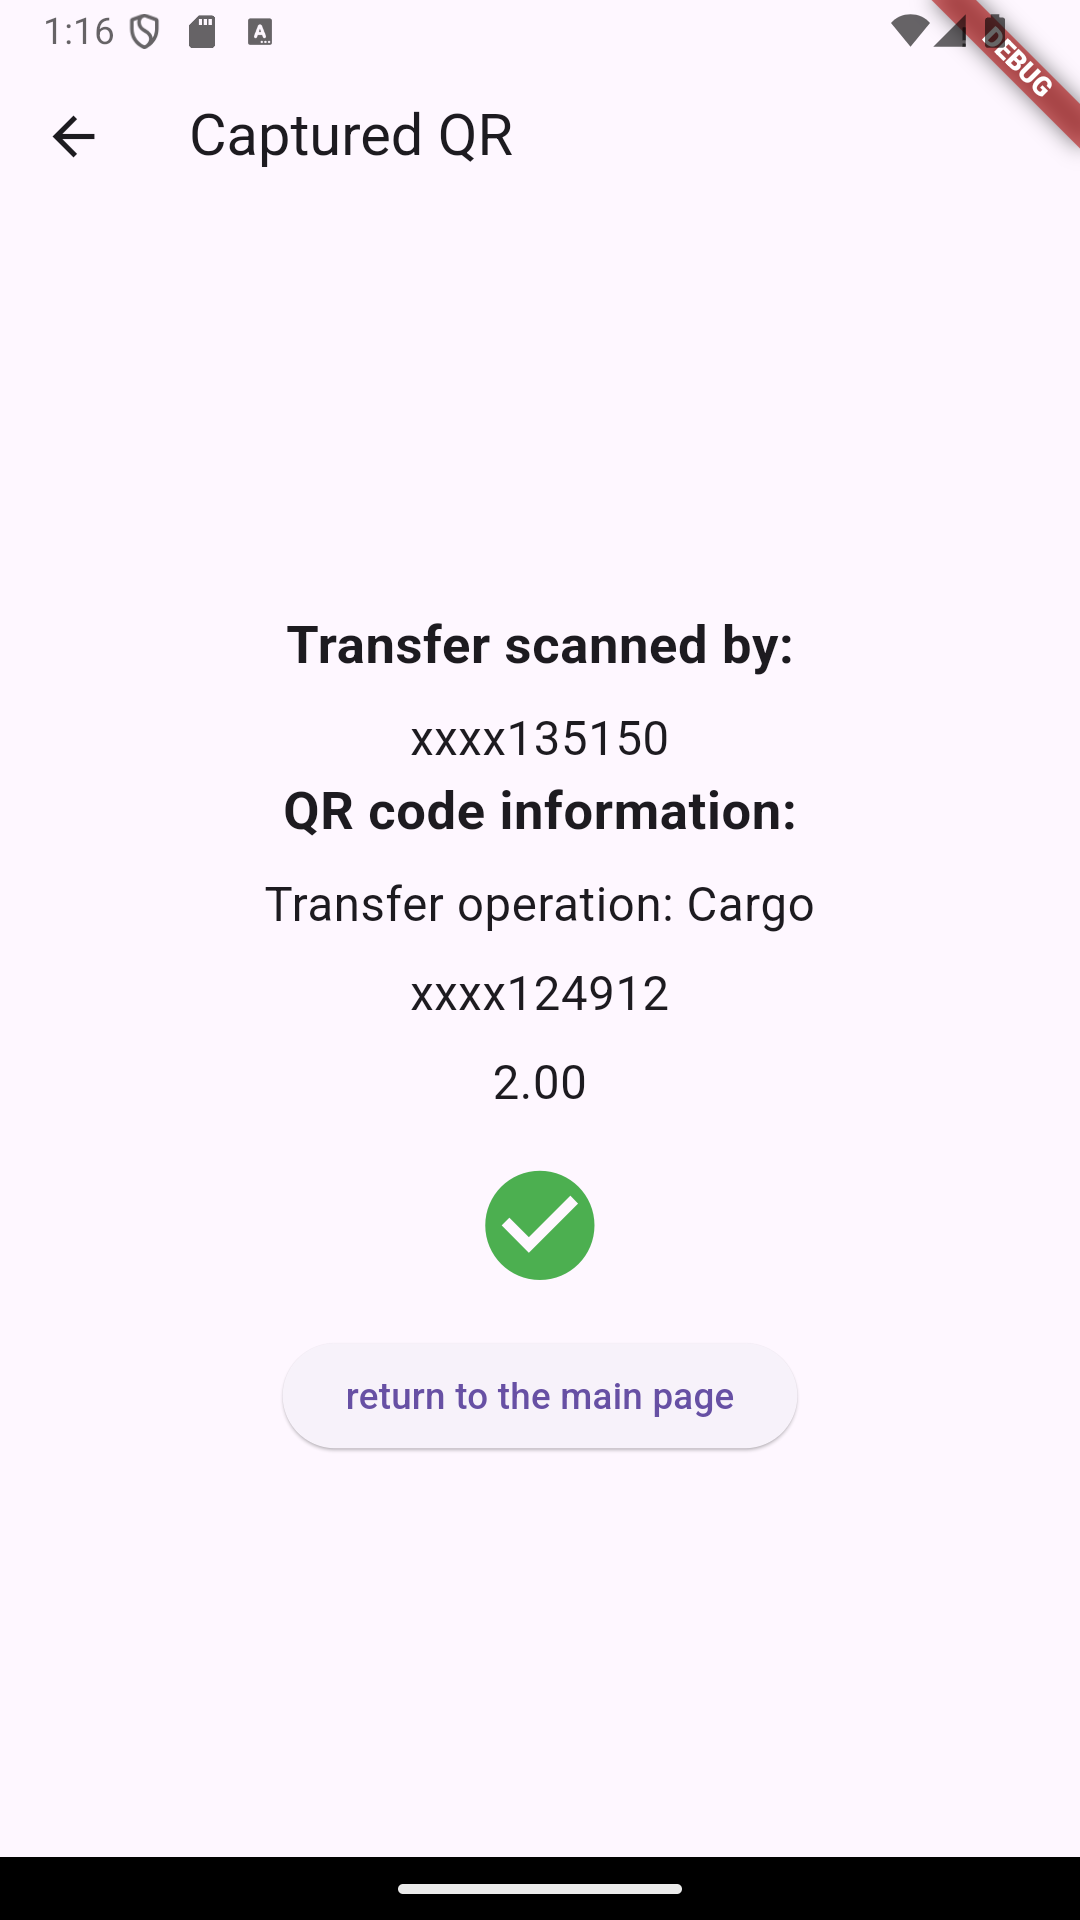
\includegraphics[width=0.3\textwidth]{imatges/capturedQR.png}
    \caption{ Pàgina per escanejar codi QR }
    \label{fig: Pàgina per escanerjar codi QR }
\end{figure}




\clearpage
\subsection{Admin}
\label{subsec: Admin}


\begin{figure}[h]
    \centering
    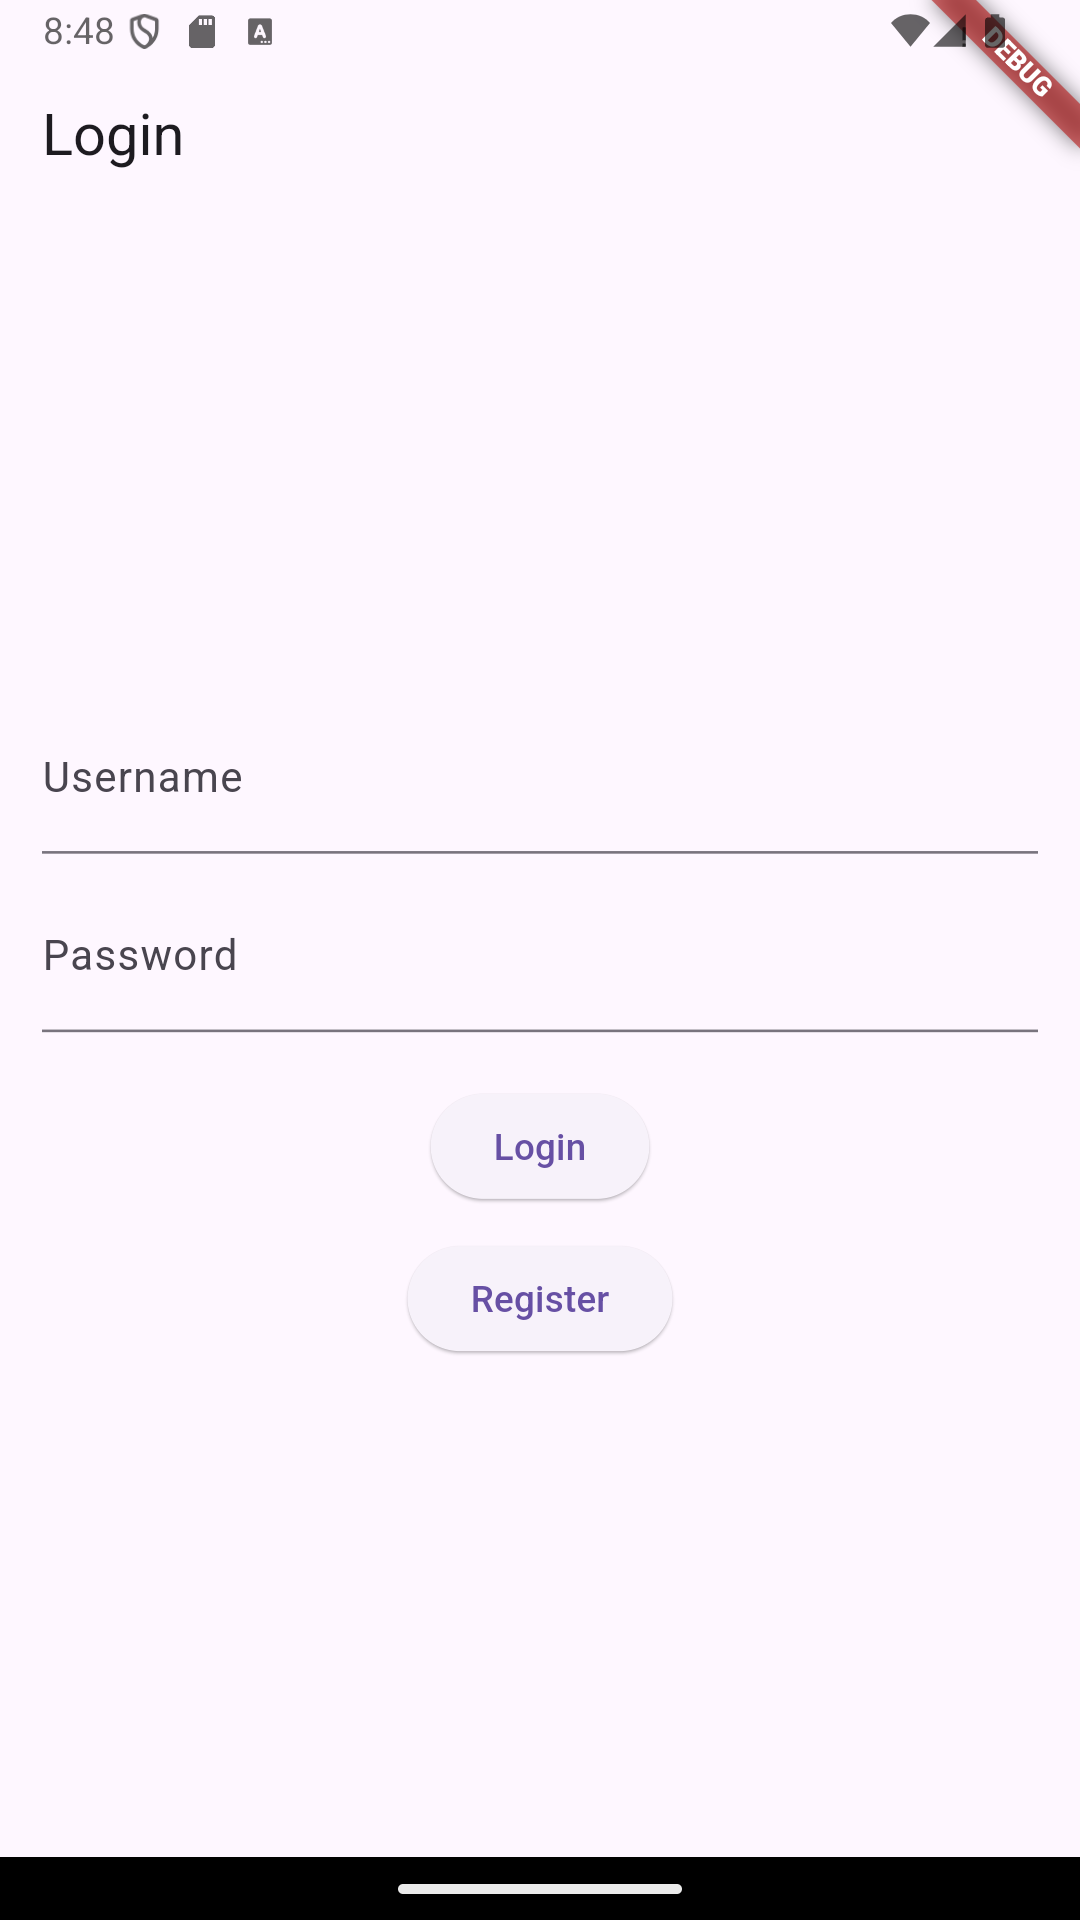
\includegraphics[width=0.3\textwidth]{imatges/login.png}
    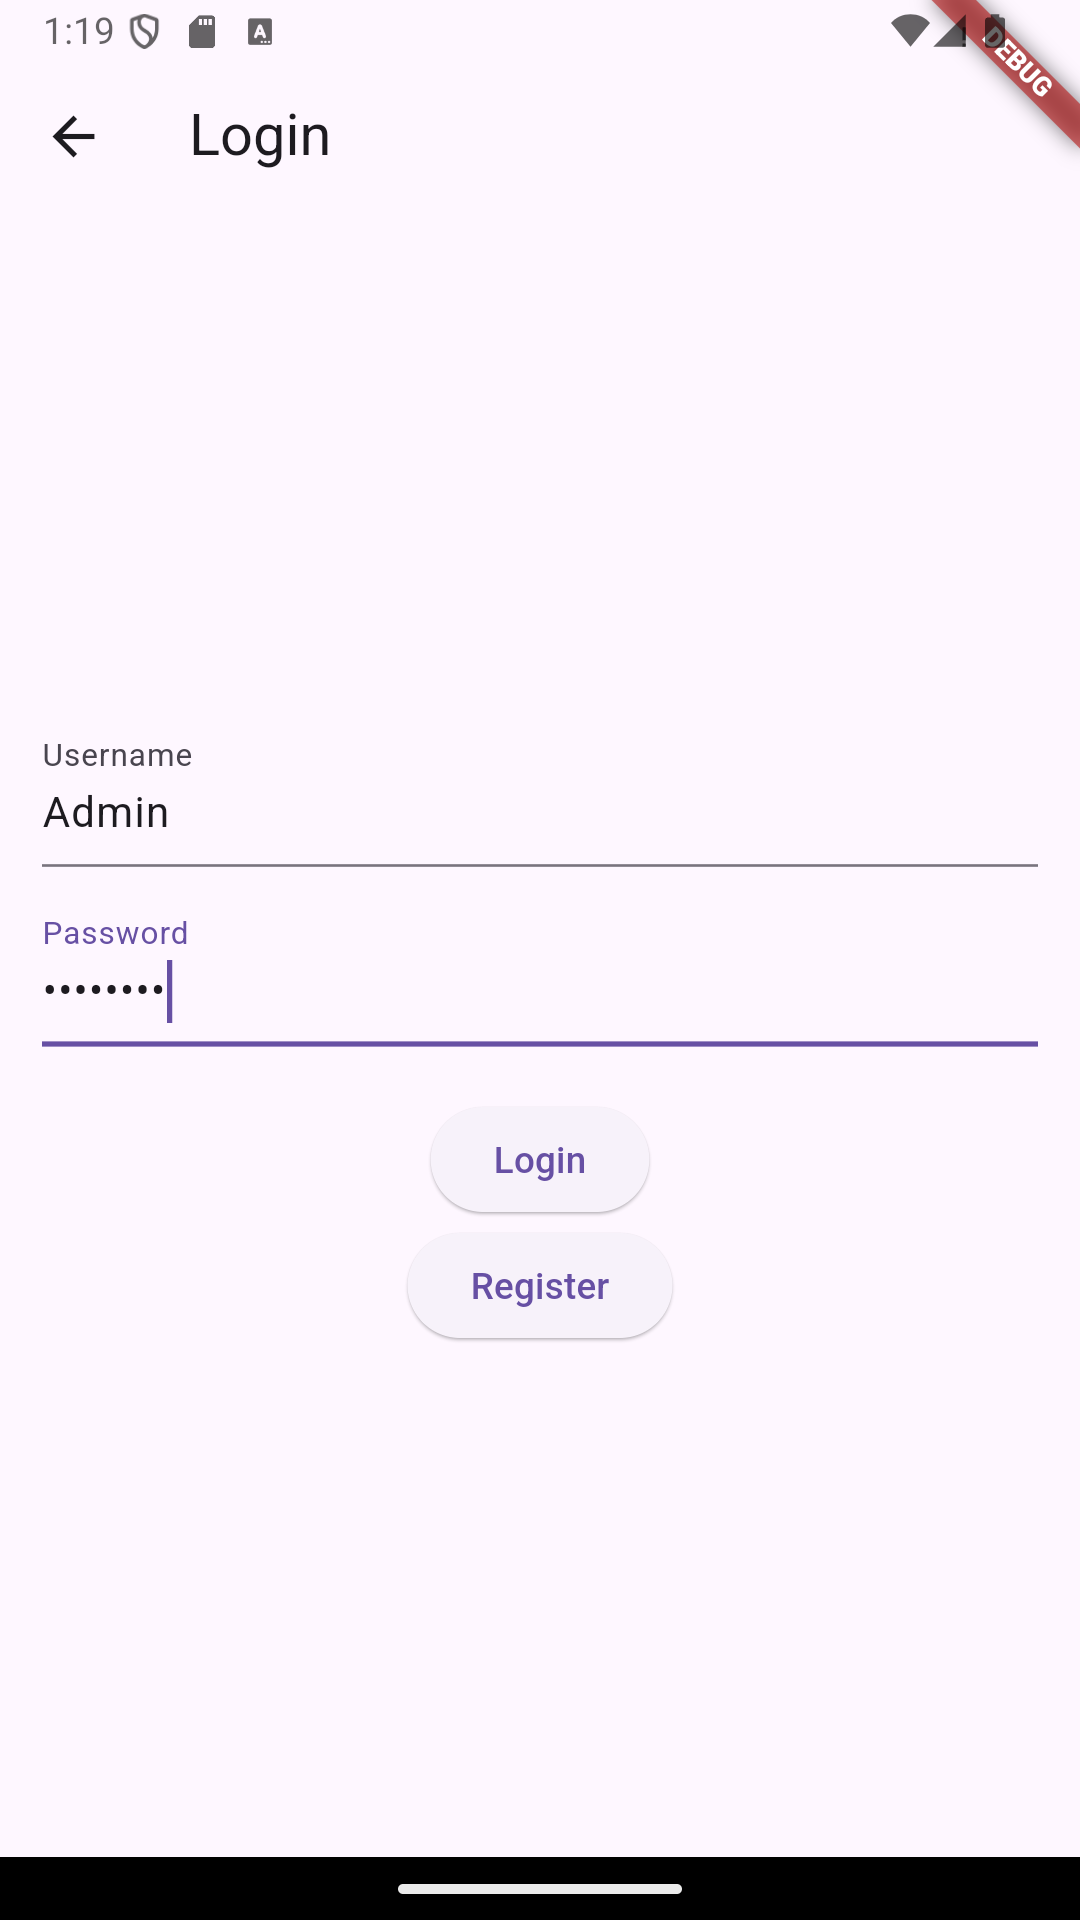
\includegraphics[width=0.3\textwidth]{imatges/loginAdmin.png}
    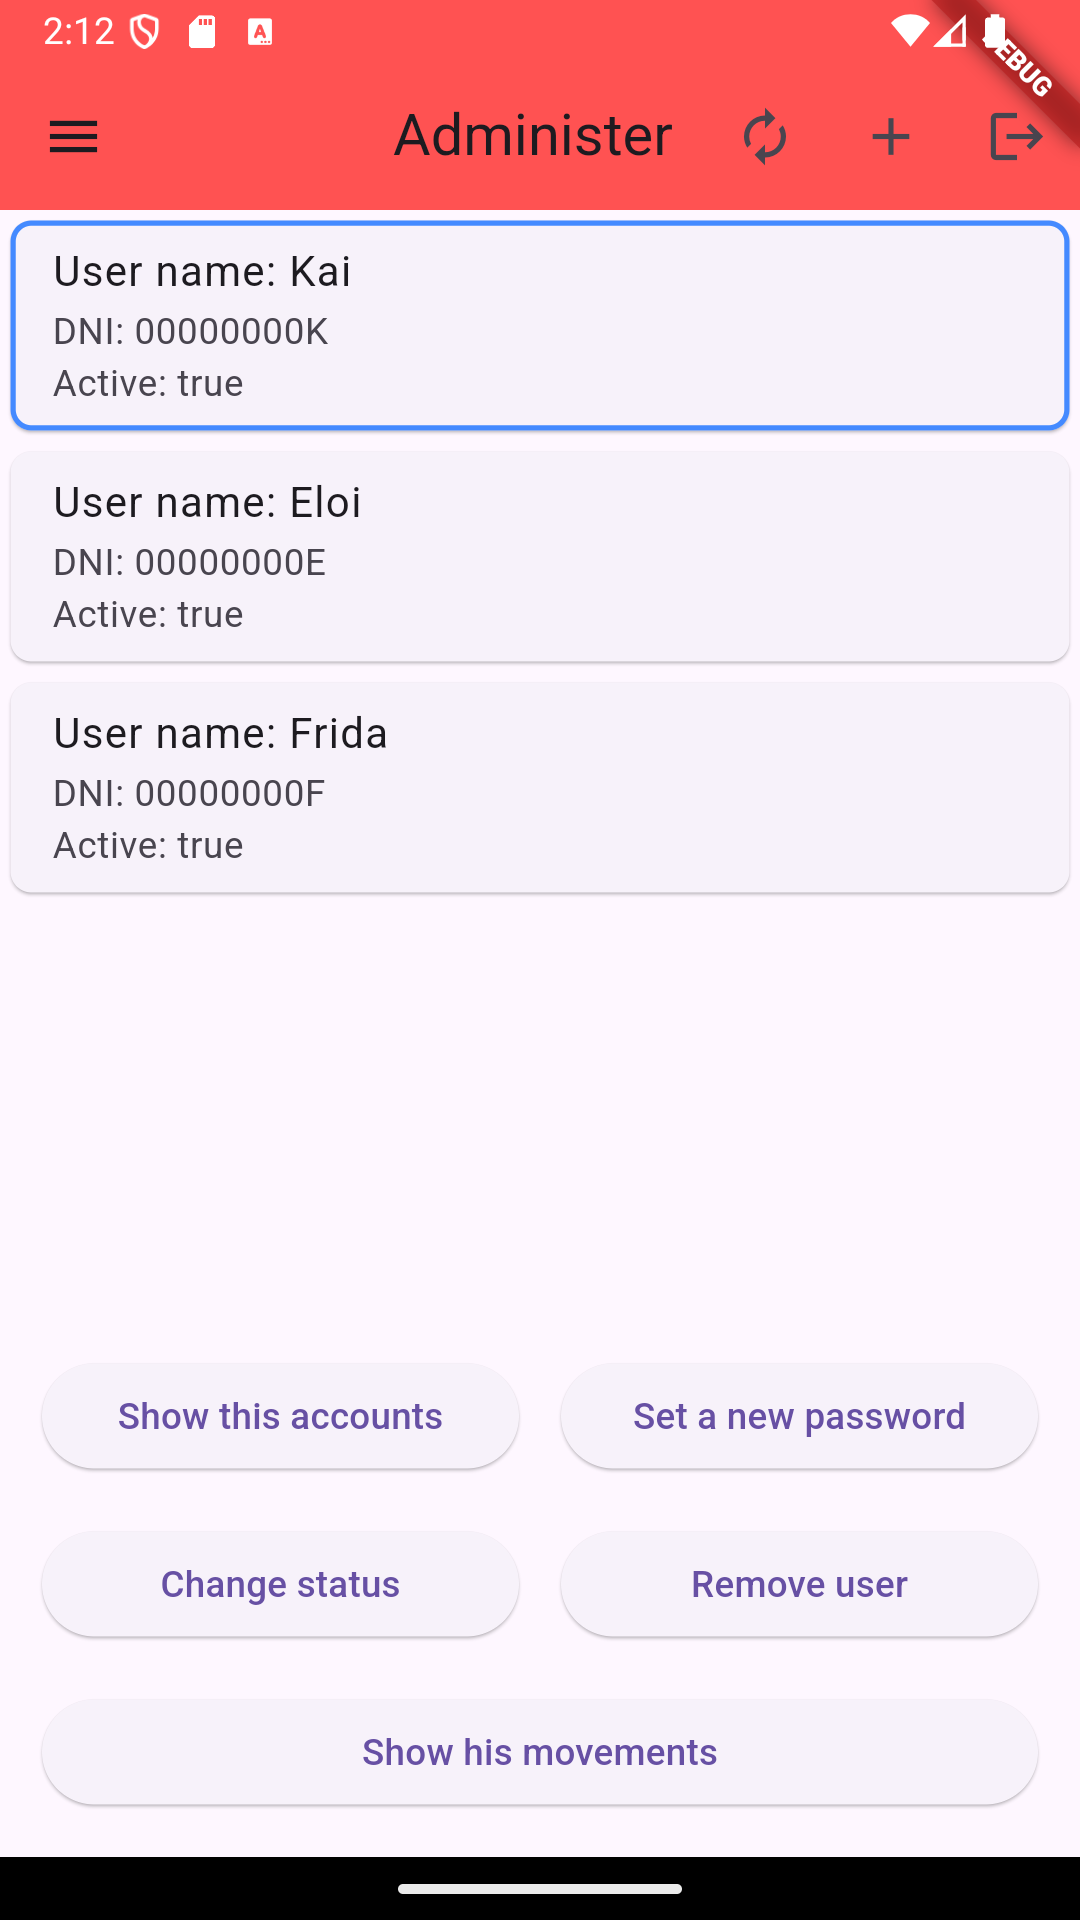
\includegraphics[width=0.3\textwidth]{imatges/administer.png}
    \caption{ Pàgina de login - Admin}
    \label{fig: Pàgina de login - Admin}
\end{figure}

\clearpage

\section{ Diagrama de processos }
\label{ sec: Diagrama de processos }


\begin{figure}[h]
    \centering
    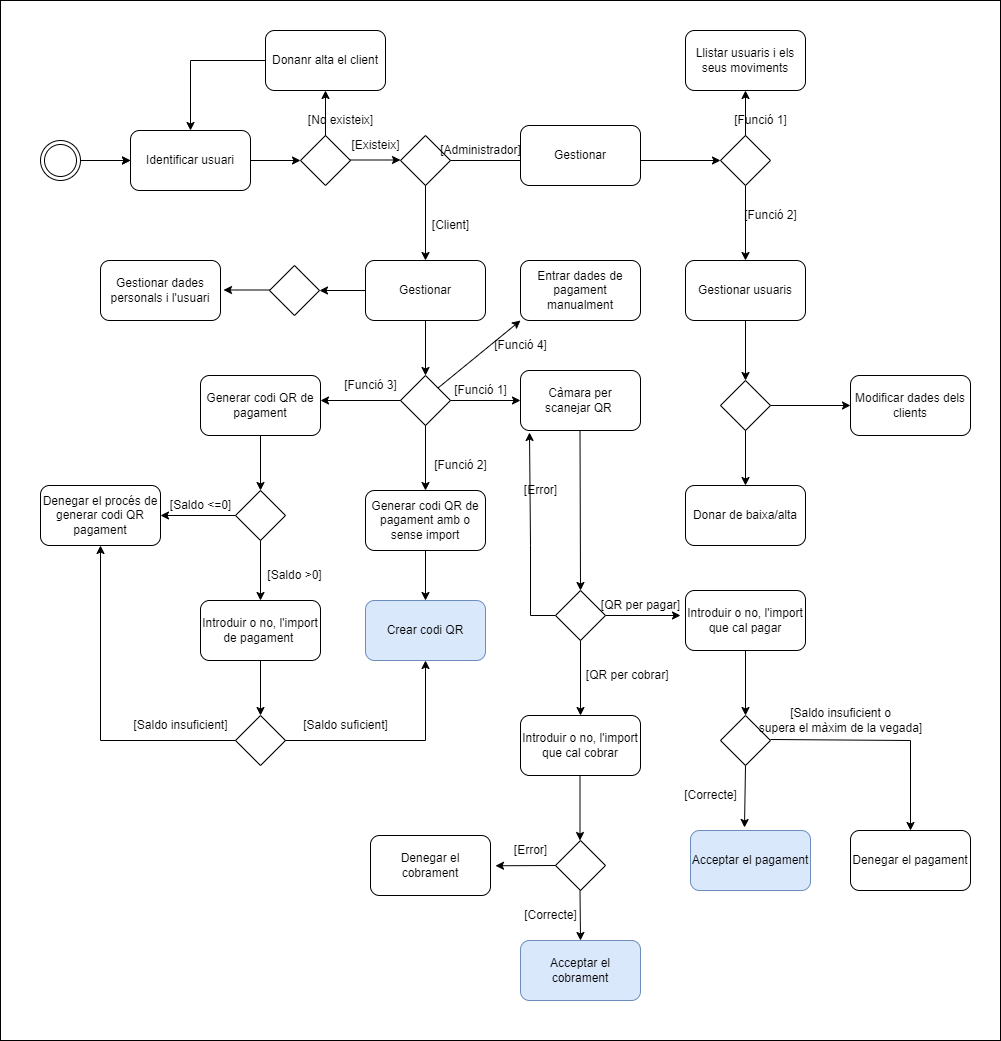
\includegraphics[width=1\textwidth]{imatges/diagrama processos.png}
    \caption{ Diagrama de processos }
    \label{fig: Diagrama de processos }
\end{figure}

Aquesta diagrama de flux representa els processos de gestió d'usuaris i transaccions de pagament mitjançant codis QR. Mostra com les diferents decisions i funcions es ramifiquen en funció de les característiques i accions de l'usuari, garantint que cada procés es gestiona adequadament segons les condicions del sistema.


\subsection{Descripció del procés}
\label{subsec:Descripció del procés}


\begin{itemize}
    \item \textbf{Identificació de l'usuari}: El procés comença amb la identificació de l'usuari. Si l'usuari no existeix, es procedeix a \textbf{donar d'alta el client}. Si l'usuari existeix, es determina si és un \textbf{Administrador} o un \textbf{Client}.
    
    \item \textbf{Administradors}: 
    \begin{itemize}
        \item \textbf{Funció 1}: Permet \textbf{llistar usuaris i els seus moviments}.
        \item \textbf{Funció 2}: Permet \textbf{gestionar usuaris}, amb accions com \textbf{modificar les dades dels clients} o \textbf{donar-los d'alta o de baixa}.
    \end{itemize}
    
    \item \textbf{Clients}: 
    \begin{itemize}
        \item Si l'usuari és un client, té l'opció de \textbf{gestionar les seves dades personals i d'usuari}.
        \item També pot optar per \textbf{entrar les dades de pagament manualment}, una solució en cas que la càmera no funcioni.
        \item \textbf{Funcions 2 i 3}: S'utilitzen per generar el codi QR de cobrament i de pagament. En cas de cobrament, no cal fixar res, però en cas de pagament, cal verificar si el compte disposa de saldo suficient. Un cop generat el codi QR, la càmera entra en joc per escanejar-lo.
        \item \textbf{Funció 1}: La càmera s'encarrega de llegir el text que hi ha darrere del codi QR i, si el missatge és correcte, processa l'operació.
        \item Cal destacar que es pot introduir l'import tant en el moment de generar el codi QR com després d'escanejar-lo.
    \end{itemize}
\end{itemize}




\chapter{Implementació i proves}
\label{chp:implementacio}


\section{Introducció}
\label{sec: Introducció}

L'objectiu d'aquest capítol és explicar el procés de desenvolupament, des del pensament
de l'aplicació i la seva estructura, al desenvolupament actual de la mateixa. També ho serà
incloure i explicació de com l'aplicació s'ha provat constantment.


\section{Organitza la idea}
\label{sec: Organitza la idea}

Quan em va ocórrer la idea de l'aplicació, vaig acabar amb una barreja de pensaments i conceptes que necessitaven ser organitzats i connectats de manera coherent. El primer pas en aquest procés va ser redactar una explicació detallada de l'aplicació, incloent l'objectiu general, les funcionalitats principals que hauria d'oferir, així com les limitacions i allò que no inclouria. Va ser essencial intentar cobrir tants detalls com fos possible per assegurar una comprensió clara del projecte.\\

Durant aquesta fase, vaig analitzar com cada component de l'aplicació es relacionava amb els altres i com s'integraria dins del sistema global. Vaig considerar les possibles interaccions entre les diferents funcionalitats i com aquestes podrien impactar l'experiència de l'usuari. A més, vaig revisar diversos enfocaments arquitectònics per determinar el més adequat per aconseguir els objectius establerts.\\

Tot i que probablement canviaria l'estructura en el futur en resposta a noves necessitats o oportunitats de millora, la idea inicial de l'arquitectura va ser útil per establir una base sòlida. A partir d'aquesta base, vaig poder començar a especificar els requisits funcionals i no funcionals de manera més detallada. Aquesta etapa va ser probablement la tasca més exigent del projecte, ja que requerí una atenció meticulosa a cada aspecte del disseny i l'estructura, a més de l'organització dels paquets de treball. Ara que aquestes parts estaven definides i estructurades, vaig poder visualitzar un full de ruta clar i detallat per al desenvolupament del sistema, el que em va permetre avançar amb una estratègia ben definida i metòdica.

\section{Desenvolupament d'aplicació}
\label{sec: Desenvolupament d'aplicació}


Vaig començar a desenvolupar l'aplicació API, ja que això ajudava a definir la base de dades. La meva estratègia consistia a implementar primer les funcionalitats més crítiques i bàsiques, assegurant-me que cada component essencial funcionés correctament abans de passar a les següents etapes. Per exemple, vaig començar amb l'operació de transacció entre dues comptes bancàries, assegurant-me que aquest procés fonamental fos fiable. Un cop aquesta funcionalitat estava operativa, vaig afegir seguretat amb l'encriptació de dades. Posteriorment, vaig implementar controls addicionals, com ara verificar si un compte disposava de saldo suficient i comprovar si el compte estava actiu.\\

Un cop vaig tenir una base sòlida al servidor, vaig començar a dissenyar la interfície d'usuari. Durant aquest procés, vaig adaptar el disseny en funció dels punts finals disponibles i les funcionalitats implementades en el servidor, mentre identificava les possibles mancances en l'API. Així, després de completar el disseny de la interfície, vaig tornar a l'API per afegir les funcionalitats que faltaven i per netejar el codi existent.\\

A mesura que avançava en el desenvolupament, vaig començar a treballar en les aplicacions d'interfície d'usuari. Vaig desenvolupar primer l'aplicació bàsica, que contenia la major part de la lògica i complexitat. Aquesta fase va ser crucial, ja que vaig afegir diversos components i vistes que posteriorment es reutilitzarien a l'aplicació client. Vaig adoptar un enfocament iteratiu: cada vegada que afegia o ajustava una funcionalitat en el servidor, feia el mateix en el client, variant les funcionalitats de manera sincronitzada. Aquesta estratègia em va permetre assegurar-me que ambdues parts de l'aplicació estiguessin alineades i funcionessin conjuntament.\\

Encara que no vaig utilitzar eines específiques com Nx, vaig intentar abstraure i reutilitzar el codi de manera eficaç per simplificar el desenvolupament. Si en el futur es necessita afegir una altra aplicació, el procés serà més senzill, ja que molts components i funcions podrien ser reutilitzats.


\section{Proves}
\label{sec: Proves}

Aquest document descriu diverses categories de proves que es duen a terme durant el desenvolupament de programari per assegurar la seva qualitat i el correcte funcionament. A continuació es presenta un breu resum de cada tipus de prova:

\begin{itemize}
\item \textbf{Proves d'unitat}: Aquestes proves se centren en verificar el correcte funcionament de les parts més petites del codi, com funcions o mètodes, de manera independent.
\item \textbf{Proves d'integració}: L'objectiu d'aquestes proves és assegurar que les diferents unitats de codi treballin bé conjuntament quan es combinen, garantint així el bon funcionament del sistema en el seu conjunt.
\item \textbf{Proves de regressió}: Aquestes proves es realitzen per garantir que les noves funcionalitats o canvis no han introduït errors en altres parts del sistema. Es tornen a executar proves prèvies per assegurar que el comportament del sistema no ha canviat de manera inesperada.
\item \textbf{Proves de sistema}: Aquestes proves verifiquen que tot el sistema compleixi amb els requisits establerts, utilitzant escenaris d'ús que reflecteixen situacions reals.
\item \textbf{Proves d'acceptació de l'usuari}: Aquestes proves són realitzades per usuaris finals en un entorn que simula el real, per obtenir el seu feedback sobre la usabilitat i l'adequació de les noves funcionalitats.
\item \textbf{Proves de càrrega i rendiment}: Es realitzen per avaluar com es comporta el sistema sota condicions de càrrega elevades i diferents situacions de rendiment, ajudant a identificar possibles problemes i millores necessàries.
\item \textbf{Proves de seguretat}: Aquestes proves tenen l'objectiu de verificar que el sistema és segur i està protegit contra vulnerabilitats i atacs potencials.
\item \textbf{Proves de compatibilitat}: S'utilitzen per assegurar que el sistema funcioni correctament en diverses plataformes, navegadors, dispositius i sistemes operatius.
\end{itemize}

L'aplicació de la interfície d'usuari (IU) s'ha provat manualment per trobar errors. En el cas de l'API, provar els punts finals ha estat una mica més difícil, però s'ha utilitzat programari especialitzat per fer-ho. Pel que fa a les aplicacions d'interfície d'usuari, s'han provat casos avançats executant l'aplicació. Quan s'ha trobat un error, primer he revisat les proves per veure si el cas no estava cobert o si va ser un error en la prova, ja que és una situació que pot passar. Si es trobava un error en les proves, vaig actualitzar les proves i després vaig corregir el codi real. Si no es trobava un error en les proves, buscaria l'error en el codi i després el cobriria amb les proves.




\chapter{Implantació i resultats}
\label{chp:implantacio}


\section{Implantació}
\label{sec: Implantació}

L'implantació de l'aplicació es realitza en diverses fases, amb un enfocament gradual per assegurar la qualitat i funcionalitat del sistema. La fase inicial del projecte va consistir en desenvolupar l'aplicació de pagament mitjançant codi QR. Aquesta primera etapa es va centrar en establir la infraestructura bàsica necessària per generar i escanejar codis QR associats a transaccions de pagament.\\

Un cop l'aplicació va estar operativa amb les funcionalitats bàsiques, la següent etapa va ser la incorporació d'una passarel·la de pagament. Aquesta passarel·la és crucial per processar les transaccions de pagament de manera segura i eficient. Actualment, el desenvolupament de la passarel·la està en curs, i la seva integració és el següent pas important per completar l'implantació de l'aplicació.\\

El projecte té dues vies potencials per a la seva implantació futura. La primera opció és integrar l'aplicació amb els sistemes bancaris estatals, similar a com funciona Bizum. Aquesta integració permetria que l'aplicació ofereixi funcionalitats similars a les d'un servei de pagament a través de bancs. La segona opció és establir una passarel·la de pagament pròpia, creant una solució similar a PayPal que permeti operar com una empresa de pagaments independent. Aquesta opció ofereix una major autonomia i flexibilitat en la gestió de les transaccions.


\section{Resultats}
\label{sec: Resultats}

Fins al moment, l'aplicació ha aconseguit implementar les funcionalitats bàsiques necessàries per generar i escanejar codis QR. No obstant això, encara falta integrar la passarel·la de pagament per completar el procés de pagament. La principal dificultat actual és la integració amb la passarel·la, que requereix una coordinació complexa amb els proveïdors de serveis de pagament i la implementació de mesures de seguretat addicionals.\\

Els beneficis esperats de l'aplicació són significatius. Un cop completada, l'aplicació permetrà als usuaris realitzar pagaments de manera senzilla i segura utilitzant codi QR, amb opcions tant per integrar-se amb bancs com per utilitzar una passarel·la de pagament pròpia. Aquesta flexibilitat en els mètodes de pagament oferirà una alternativa valuosa a serveis establerts com PayPal i proporcionarà als usuaris una solució innovadora i eficient per als seus pagaments.\\

Els pròxims passos en el desenvolupament inclouen la finalització de la integració de la passarel·la de pagament i la implementació de les funcionalitats avançades. A continuació, es realitzaran proves exhaustives per garantir el bon funcionament del sistema abans del llançament oficial de l'aplicació.



\section{Prova 1}
\section{Prova 2}
\section{Prova 3}
\section{Prova 4}
\section{Prova 5}
\section{Prova 6}
\section{Prova 7}
\section{Prova 8}
\section{Prova 9}
\section{Prova 10}
\section{Prova 11}





\chapter{Conclusions}
\label{chp:conclusions}


L'objectiu d'aquest projecte és permetre que les persones puguin realitzar operacions bancàries amb la màxima flexibilitat i seguretat possible. La idea va sorgir després de la meva experiència a la Xina el 2019, on vaig observar que la majoria de les transaccions es realitzaven a través de l'aplicació de missatgeria "WeChat". Aquesta aplicació integra una passarel·la de pagament molt còmoda, que facilita les transaccions i ofereix una major transparència en les operacions. A més, l'ús de pagaments electrònics contribueix a reduir els robatoris associats amb l'ús de diners en efectiu.\\

Recentment, vaig visitar una sala de jocs amb amics on vaig notar un canvi significatiu en el sistema de pagament. Abans, només es podien utilitzar monedes de 1€ per activar les màquines, però ara s'ha afegit un mini TPV per a cada màquina. Aquesta actualització requereix una inversió en infraestructura per als TPV. Imagina si aquest procés es pogués simplificar utilitzant un codi QR: cada màquina podria estar configurada amb l'import a cobrar, mentre que els clients podrien pagar fàcilment escanejant el codi QR a través del seu dispositiu mòbil. Aquesta solució ofereix una alternativa més flexible i eficient, tant per a les empreses com per als usuaris.\\


El sistema de pagament amb codi QR ofereix una sèrie d'avantatges clau. En primer lloc, simplifica el procés de pagament, ja que els clients poden realitzar transaccions simplement escanejant un codi QR amb el seu dispositiu mòbil. Això redueix la necessitat d'infraestructura física com terminals de punt de venda (TPV) i minimitza els problemes associats amb el seu manteniment, com ara problemes de bateria, cobertura o maquinari defectuós.\\

Tanmateix, per adoptar amb èxit aquesta tecnologia, cal avançar en diversos aspectes. En primer lloc, és essencial garantir la seguretat de les transaccions. El procés de pagament amb codi QR ha d'incloure mesures de seguretat robustes, com l'encriptació de dades i l'autenticació de dos factors, per protegir les dades dels usuaris i prevenir fraus.\\

A més, la implementació d'una passarel·la de pagament fiable i eficient és crucial. Això pot implicar la integració amb sistemes de pagament establerts, com Bizum, o el desenvolupament d'una solució pròpia, similar a PayPal. La passarel·la de pagament ha de ser capaç de gestionar les transaccions de manera fluida i assegurar la compatibilitat amb diversos dispositius i aplicacions.\\


En resum, els pagaments mitjançant codi QR poden revolucionar la forma en què es realitzen les transaccions comercials, oferint una solució més flexible i eficient. Encara que plantegen nous reptes, especialment en termes de seguretat, la continuïtat en la innovació tecnològica pot ajudar a superar aquests obstacles i millorar l'experiència de pagament per a usuaris i negocis per igual.\\




\chapter{Treball futur}
\label{chp:treballfutur}



\section{Funcionalitats de l'aplicació}
\label{sec: Funcionalitats de l'aplicació}

A més, com a funcionalitats futures, tot i que no són prioritàries en aquesta fase inicial del projecte, el sistema podria incloure:

\begin{itemize}
\item Una pàgina d'anàlisi que proporcioni informació detallada sobre les transaccions realitzades, ajudant els comerciants a gestionar millor les seves vendes.
\item Un sistema de subscripcions que permeti als clients realitzar pagaments recurrents de manera automàtica.
\item Millores en els aspectes visuals per a una millor experiència d'usuari.
\item Incorporar notificacions per veu quan es realitzi una transacció bancària, millorant així la facilitat d'ús i el seguiment en temps real.
\end{itemize}

Aquestes funcionalitats addicionals estan pensades per ampliar les capacitats del sistema i oferir un valor afegit tant als usuaris, contribuint així a una experiència de pagament més fluida i moderna.

\section{Seguretat de dades}
\label{sec: Seguretat de dades}

Un aspecte clau a destacar és el sistema d'encriptació. Actualment he utilitzat l'encriptació AES (Advanced Encryption Standard), que és un algorisme de xifrat simètric àmpliament utilitzat per la seva eficàcia i seguretat. No obstant això, considero que seria molt més avantatjós implementar l'encriptació RSA (Rivest-Shamir-Adleman), que és un sistema d'encriptació asimètric. L'encriptació RSA utilitza un parell de claus, una pública i una privada, per assegurar les dades, oferint un nivell de seguretat addicional en comparació amb AES. Això permet una gestió més segura de les claus i millora la protecció de les transaccions en línia.


\section{Millora del codi}
\label{sec: Millora del codi}


En el codi actual hi ha molts aspectes que es poden millorar, així com nombrosos fragments de codi repetits que es podrien optimitzar. En el futur, es recomana refactoritzar el codi per millorar la seva eficiència i mantenibilitat. També seria molt important afegir tests per validar el codi freqüentment, utilitzant frameworks com Nx.



\chapter{Bibliografia}
\label{chp:Bibliografia}



% \backmatter % From this point, chapters are unnumbered


%%%%%%%%%%%%%%%%%%%%%%%%%%%%%%%%%%%%%%%%%%%%
% GETI projects: bibliography as a chapter
%%%%%%%%%%%%%%%%%%%%%%%%%%%%%%%%%%%%%%%%%%%%
%\chapter{Bibliografia}
%\renewcommand{\bibsection}{} % Remove intrinsic bibliography name

\bibliographystyle{ThesisStyleBreakable}
\bibliography{bibliography}

%%%%%%%%%%%%%%%%%%%%%%%%%%%%%%%%%%%%%%%%%%%%
% GETI projects: move "\backmatter" after bibliography to allow unnumbered appendices
%%%%%%%%%%%%%%%%%%%%%%%%%%%%%%%%%%%%%%%%%%%%
% \backmatter



% APPENDICES

% 1. Short and limited command for appendices:
% \appendix

% 2. Full command for appendices (package 'appendices' needed in the preamble: check 'thesis-style.sty'):
% \usepackage[title]{appendix} % add 'titletoc' to add "Appendix" to ToC

% \begin{appendices}

% To manually set appendix chapter names (should be after "\backmatter"):
% \renewcommand{\chaptermark}[1]{\markboth{#1}{}}
% \chapter{Appendix A. Appendix name}

% To let the package manage appendix chapter names (before "\backmatter"):
% \chapter{Appendix name}

% Alternative for separated appendices:
% \include{Appendix1}

% \end{appendices}

% 3. No command for appendices (just unnumbered chapters):
% \renewcommand{\chaptermark}[1]{\markboth{#1}{}}
% \chapter{Appendix A. Appendix name}


%%%%%%%%%%%%%%%%%%%%%%%%%%%%%%%%%%%%%%%%%%%%
% GETI projects: change header to show appendix mark
%%%%%%%%%%%%%%%%%%%%%%%%%%%%%%%%%%%%%%%%%%%%
% \fancyhead[RE,LO]{\bfseries\color{black}\appendixmark}    % Appendix mark (boldface) in the right on even pages, and in the left on odd pages


\renewcommand\appendixname{Annex} % Appendix name (change default)

\begin{appendices}

\chapter{Pressupost}

Lorem ipsum dolor sit amet, consectetur adipiscing elit. Nunc congue mattis tellus, in rhoncus nisl laoreet vel. Sed nulla libero, tincidunt id ligula congue, hendrerit maximus mi. Morbi nec metus in urna imperdiet mattis pretium a libero. Fusce est mauris, convallis id facilisis faucibus, consequat aliquet eros. Vivamus et dui pulvinar, rutrum velit at, volutpat tellus. Nulla vehicula ullamcorper justo, blandit interdum leo sagittis quis. Quisque convallis vel ante ac rutrum. Morbi et varius sem, sed tristique elit. Vestibulum aliquam facilisis pellentesque. Suspendisse consequat commodo eros, sit amet tincidunt sapien semper in. Nunc ut magna ac quam tempor malesuada et at ex. Donec mattis mauris ante, id condimentum elit dapibus at.

Curabitur ut sodales sapien. Etiam eget ultrices risus, in dignissim nunc. Quisque quis tortor in nunc posuere lacinia ut sed dui. Praesent ut sollicitudin diam, ut mattis magna. Morbi porttitor fermentum magna a pharetra. Nullam at magna diam. Suspendisse vehicula tellus eget ligula aliquam semper. Integer sed ullamcorper felis, ac imperdiet elit. Praesent eu suscipit ligula, sit amet vulputate erat. Etiam eget tempor est, vitae aliquet tortor. Nam efficitur tristique ligula. Aliquam blandit leo non ante suscipit, vitae mattis diam rhoncus. Ut ac dui sit amet dui venenatis suscipit.

Nunc sollicitudin hendrerit risus, quis ultricies orci elementum non. Aliquam erat volutpat. Mauris neque turpis, molestie in tellus id, pharetra gravida mi. Suspendisse potenti. Donec aliquam dolor eu pellentesque auctor. Proin eget sapien ut tellus maximus lacinia. Praesent blandit pretium mi, suscipit sollicitudin eros iaculis in. Nunc a justo sit amet mauris auctor posuere sit amet vel erat. Etiam in maximus nisi. Pellentesque blandit pharetra lectus nec efficitur. Praesent tristique vel arcu id bibendum. In eget eros fringilla magna hendrerit facilisis ac vitae urna. Donec malesuada fermentum dictum. Pellentesque aliquet tortor vitae suscipit tempus. Phasellus ornare risus mi, vel placerat justo efficitur eu. Phasellus quis tincidunt enim.

Etiam a elementum lorem. Integer ac lectus hendrerit, venenatis ante vitae, accumsan eros. Orci varius natoque penatibus et magnis dis parturient montes, nascetur ridiculus mus. Curabitur non varius dolor. Donec suscipit metus vitae ultrices sagittis. Praesent ac dapibus justo, vel mollis sapien. Pellentesque at iaculis neque. Donec ac tellus orci. Pellentesque eleifend fringilla massa, in lobortis nibh finibus in. Morbi ut neque vitae est congue tempor efficitur imperdiet dolor. Pellentesque nec nibh nec nibh fringilla laoreet. Duis fermentum ornare sollicitudin. Maecenas finibus tincidunt justo commodo commodo. Suspendisse venenatis odio dignissim auctor elementum. Duis non mauris orci.

Lorem ipsum dolor sit amet, consectetur adipiscing elit. Nunc congue mattis tellus, in rhoncus nisl laoreet vel. Sed nulla libero, tincidunt id ligula congue, hendrerit maximus mi. Morbi nec metus in urna imperdiet mattis pretium a libero. Fusce est mauris, convallis id facilisis faucibus, consequat aliquet eros. Vivamus et dui pulvinar, rutrum velit at, volutpat tellus. Nulla vehicula ullamcorper justo, blandit interdum leo sagittis quis. Quisque convallis vel ante ac rutrum. Morbi et varius sem, sed tristique elit. Vestibulum aliquam facilisis pellentesque. Suspendisse consequat commodo eros, sit amet tincidunt sapien semper in. Nunc ut magna ac quam tempor malesuada et at ex. Donec mattis mauris ante, id condimentum elit dapibus at.

Curabitur ut sodales sapien. Etiam eget ultrices risus, in dignissim nunc. Quisque quis tortor in nunc posuere lacinia ut sed dui. Praesent ut sollicitudin diam, ut mattis magna. Morbi porttitor fermentum magna a pharetra. Nullam at magna diam. Suspendisse vehicula tellus eget ligula aliquam semper. Integer sed ullamcorper felis, ac imperdiet elit. Praesent eu suscipit ligula, sit amet vulputate erat. Etiam eget tempor est, vitae aliquet tortor. Nam efficitur tristique ligula. Aliquam blandit leo non ante suscipit, vitae mattis diam rhoncus. Ut ac dui sit amet dui venenatis suscipit.

Nunc sollicitudin hendrerit risus, quis ultricies orci elementum non. Aliquam erat volutpat. Mauris neque turpis, molestie in tellus id, pharetra gravida mi. Suspendisse potenti. Donec aliquam dolor eu pellentesque auctor. Proin eget sapien ut tellus maximus lacinia. Praesent blandit pretium mi, suscipit sollicitudin eros iaculis in. Nunc a justo sit amet mauris auctor posuere sit amet vel erat. Etiam in maximus nisi. Pellentesque blandit pharetra lectus nec efficitur. Praesent tristique vel arcu id bibendum. In eget eros fringilla magna hendrerit facilisis ac vitae urna. Donec malesuada fermentum dictum. Pellentesque aliquet tortor vitae suscipit tempus. Phasellus ornare risus mi, vel placerat justo efficitur eu. Phasellus quis tincidunt enim.

Etiam a elementum lorem. Integer ac lectus hendrerit, venenatis ante vitae, accumsan eros. Orci varius natoque penatibus et magnis dis parturient montes, nascetur ridiculus mus. Curabitur non varius dolor. Donec suscipit metus vitae ultrices sagittis. Praesent ac dapibus justo, vel mollis sapien. Pellentesque at iaculis neque. Donec ac tellus orci. Pellentesque eleifend fringilla massa, in lobortis nibh finibus in. Morbi ut neque vitae est congue tempor efficitur imperdiet dolor. Pellentesque nec nibh nec nibh fringilla laoreet. Duis fermentum ornare sollicitudin. Maecenas finibus tincidunt justo commodo commodo. Suspendisse venenatis odio dignissim auctor elementum. Duis non mauris orci.

Lorem ipsum dolor sit amet, consectetur adipiscing elit. Nunc congue mattis tellus, in rhoncus nisl laoreet vel. Sed nulla libero, tincidunt id ligula congue, hendrerit maximus mi. Morbi nec metus in urna imperdiet mattis pretium a libero. Fusce est mauris, convallis id facilisis faucibus, consequat aliquet eros. Vivamus et dui pulvinar, rutrum velit at, volutpat tellus. Nulla vehicula ullamcorper justo, blandit interdum leo sagittis quis. Quisque convallis vel ante ac rutrum. Morbi et varius sem, sed tristique elit. Vestibulum aliquam facilisis pellentesque. Suspendisse consequat commodo eros, sit amet tincidunt sapien semper in. Nunc ut magna ac quam tempor malesuada et at ex. Donec mattis mauris ante, id condimentum elit dapibus at.

Curabitur ut sodales sapien. Etiam eget ultrices risus, in dignissim nunc. Quisque quis tortor in nunc posuere lacinia ut sed dui. Praesent ut sollicitudin diam, ut mattis magna. Morbi porttitor fermentum magna a pharetra. Nullam at magna diam. Suspendisse vehicula tellus eget ligula aliquam semper. Integer sed ullamcorper felis, ac imperdiet elit. Praesent eu suscipit ligula, sit amet vulputate erat. Etiam eget tempor est, vitae aliquet tortor. Nam efficitur tristique ligula. Aliquam blandit leo non ante suscipit, vitae mattis diam rhoncus. Ut ac dui sit amet dui venenatis suscipit.

Nunc sollicitudin hendrerit risus, quis ultricies orci elementum non. Aliquam erat volutpat. Mauris neque turpis, molestie in tellus id, pharetra gravida mi. Suspendisse potenti. Donec aliquam dolor eu pellentesque auctor. Proin eget sapien ut tellus maximus lacinia. Praesent blandit pretium mi, suscipit sollicitudin eros iaculis in. Nunc a justo sit amet mauris auctor posuere sit amet vel erat. Etiam in maximus nisi. Pellentesque blandit pharetra lectus nec efficitur. Praesent tristique vel arcu id bibendum. In eget eros fringilla magna hendrerit facilisis ac vitae urna. Donec malesuada fermentum dictum. Pellentesque aliquet tortor vitae suscipit tempus. Phasellus ornare risus mi, vel placerat justo efficitur eu. Phasellus quis tincidunt enim.

Etiam a elementum lorem. Integer ac lectus hendrerit, venenatis ante vitae, accumsan eros. Orci varius natoque penatibus et magnis dis parturient montes, nascetur ridiculus mus. Curabitur non varius dolor. Donec suscipit metus vitae ultrices sagittis. Praesent ac dapibus justo, vel mollis sapien. Pellentesque at iaculis neque. Donec ac tellus orci. Pellentesque eleifend fringilla massa, in lobortis nibh finibus in. Morbi ut neque vitae est congue tempor efficitur imperdiet dolor. Pellentesque nec nibh nec nibh fringilla laoreet. Duis fermentum ornare sollicitudin. Maecenas finibus tincidunt justo commodo commodo. Suspendisse venenatis odio dignissim auctor elementum. Duis non mauris orci.

\chapter{Planificació}


\end{appendices}

% \printnomenclature

\end{document}
